% Todo: consolidate two sets of tables for intro eg
% add small e.g. to tables, big summaryt +
% Search for !!! and TODO symbols after review

\documentclass[a4paper,10pt]{article}
\usepackage[utf8x]{inputenc}
\usepackage{natbib}
\usepackage{booktabs}
\usepackage[margin=0.9in]{geometry}
\usepackage{graphicx}
\usepackage{fancyvrb}
\usepackage{listings}
\usepackage{bm}
\usepackage{xcolor}
\usepackage{multirow}
\usepackage{booktabs}
\usepackage{placeins}

\usepackage{array}
\newcolumntype{C}[1]{>{\arraybackslash}p{#1}}

\usepackage{hyperref}
\usepackage[capitalise]{cleveref}

\xdefinecolor{gray}{rgb}{0.4,0.4,0.4}
\xdefinecolor{blue}{RGB}{58,95,205}% R's royalblue3; #3A5FCD

\lstset{% setup listings
        language=R,% set programming language
        basicstyle=\ttfamily,% basic font style
        keywordstyle=\color{blue},% keyword style
        commentstyle=\color{gray},% comment style
        numberstyle=\scriptsize,% use small line numbers
        numbersep=10pt,% space between line numbers and code
        tabsize=3,% sizes of tabs
        showstringspaces=false,% do not replace spaces in strings by a certain character
        captionpos=b,% positioning of the caption below
        breaklines=true,% automatic line breaking
        escapeinside={(*}{*)},% escaping to LaTeX
        fancyvrb=false,% verbatim code is typset by listings
        extendedchars=false,% prohibit extended chars (chars of codes 128--255)
        literate={"}{{\texttt{"}}}1{<--}{{$\bm\leftarrow$}}1{<<-}{{$\bm\twoheadleftarrow$}}1
        {~}{{$\bm\sim$}}1{<=}{{$\bm\le$}}1{>=}{{$\bm\ge$}}1{!=}{{$\bm\neq$}}1{^}{{$^{\bm\wedge}$}}1,% item to replace, text, length of chars
        alsoletter={.<-},% becomes a letter
        alsoother={$},% becomes other
        otherkeywords={!=, ~, $, \&, \%/\%, \%*\%, \%\%, <-, <<-, /},% other keywords
        deletekeywords={c}% remove keywords
}


\graphicspath{{../figure/}}

%opening
\title{Evaluating the performance of Iterative Proportional Fitting for spatial microsimulation: new tests for an established technique}
% \author{Robin Lovelace}

\begin{document}

\maketitle

\begin{abstract}
Iterative Proportional Fitting (IPF), also known as biproportional
fitting, `raking' or the RAS algorithm,
is an established procedure used in a variety of applications
across the social sciences. Primary amongst these for urban modelling has been its use in
static spatial microsimulation to generate small area microdata --- individual
level data allocated to administrative zones.
The technique is mature, widely used and relatively straight-forward.
Although IPF is well described mathematically, reproducible examples of the
algorithm, written in modern programming languages, are rare in the academic
literature. Therefore, there is  a tendency for researchers to `start from
scratch', resulting in a variety ad-hoc implementations and little evidence about the relative merits of differing approaches.
These knowledge gaps mean that answers to methodological questions must be guessed:
% Under what conditions can convergence be expected?
% How many iterations should be used for any given application? 
What impact can initial weights have on the final result?
How can `empty cells' be identified
and how do they influence model fit? Can IPF
be made more computationally efficient?
This paper tackles such questions, using a systematic methodology 
based on publicly available code and data.
The results demonstrate the sensitivity of the results to
initial conditions, notably to `empty cells', and the
importance of software choices for IPF's computational efficiency.
The paper concludes by proposing an agenda for robust and reproducible future tests
% and offers more general guidance on how
% the method can be implemented
for IPF and other methodologies used in spatial microsimulation.

Keywords: Iterative proportional fitting, spatial microsimulation, modelling

JEL Code: C
\end{abstract}

\section{Introduction}
Surveys of the composition, attitudes and behaviour of individual
respondents constitute a ubiquitous empirical basis of social science research.
The aggregation of survey data of this type also has a long history.
Generally this involves translating raw data from a `long' or `microdata' format
--- as survey information is entered into a database,
one individual at a time ---
to a `wide' data format \citep{van2012flexible}. In wide or `areal' datasets,
each row represents a contiguous and mutually exclusive geographic area
containing a subset of the total population; each column represents a
variable value or bin (\citealp{Openshaw1983}; see \cref{fmsim-schema}).
The transformation from `long' to `wide' is typically carried out
for the following reasons: to preserve anonymity of participants \citep{Lee2009,marsh1993};
to ease storage and retrieval of information ---
 aggregate-level datasets can represent information about millions of individuals
in relatively little computer disk space; and to ease the loading, visualisation and
 analysis of official data in geographical information systems (GIS).

The process of aggregation is generally performed in three steps:  % commented out as it's not amazing
\begin{enumerate}
 \item Conversion of
variables into discrete categories (e.g.~a person aged 21
could be allocated to the age band 20--25).
 \item Assignment of a column to each unique category.
% --- and in some cases each category combination ---
 \item Assignment of
integer counts to cells in each column to represent the number of people with each characteristic.
\end{enumerate}

However, the process of aggregation has some important disadvantages.
Geographically aggregated datasets are problematic for the
analysis of spatial phenomena \citep{Openshaw1984} and can prevent the analysis of
the interdependencies between individual and household variables
at the local level \citep{Lee2009}. In an effort to address the drawbacks associated with this lack of microdata,
Samples of Anonymised Records (SARs) were released from the 1991 Census
\citep{marsh1993,middleton1995samples} and this was followed by similar SARs releases in 2001 and 2011.
Nevertheless, the SARs are not suitable for intra-city and neighbourhood level
analysis, as the smallest geographical level at which such microdata are publicly
available is the Local Authority, to preserve confidentiality.
There has been discussion of ways to further disaggregate the geography
of the SARs, with due emphasis on risks to confidentiality \citep{Tranmer2005case4}.
Furthermore, there are many policy relevant variables (e.g.~income and wealth,
social attitudes) that are not collected by the Census in many countries,
making these variables
unavailable at the small area level.



% It is these disadvantages that spatial microsimulation and small
% area estimation seek to address.
One way geographers and regional scientists have addressed
these data issues and lack of small area information is through the development
and application of the overlapping methods of small area estimation and
spatial microsimulation \citep{Ballas2005c,Hermes2012a}.\footnote{There
is a great deal of overlap between methods for spatial microsimulation and
small area estimation (the terms are sometimes used
interchangeably). It is useful
to have two terms, however. Small
area estimation seeks to estimate summary statistics for a variable whose
geographical distribution is unknown, sometimes via a spatial microdataset. With spatial
microsimulation, on the other hand, the emphasis is on generating and analysing
spatial microdata.}
Spatial microsimulation combines national social survey microdata
(such as the Understanding Society panel dataset UK) with small area census data.
A number of techniques are available --- see \citet{tanton2014review} for a recent review ---
including deterministic reweighting \citep{Birkin1989a},
genetic algorithms and simulated annealing \citep{Williamson1998}
as well as approaches based on linear regression \citep{Harding2011}.
It is an active field of development with ongoing refinements
(e.g.~\citealp{Lovelace2013-trs,Pritchard2012}) and debates
about which approaches are most suited in different situations
\citep{harland2012,Hermes2012a,Smith2009,whitworth2013evaluations,Williamson2013}

These methods are important because
large national social survey datasets are often \emph{only} available in
the wide, geographically aggregated form. Information loss occurs when
georeferenced individual level survey data ---
spatial microdata --- is aggregated in this way. This problem is exacerbated
when continuous variables are converted into discrete categories and when
cross-tabulations, such as age/income, are not provided, as is often the case.

One of the key techniques used in spatial microsimulation and small area estimation is
Iterative proportional fitting (IPF). IPF can help overcome the limitations of wide,
geographically aggregated data sources when used in
\emph{spatial microsimulation}. In simplistic terms spatial microsimulation can be understood
as the reversal of geographic aggregation described in points 1--3 above,
to approximate the original `long' dataset (\cref{fmsim-schema}).
Thus the need for spatial microsimulation is driven by
the tendency of statistical agencies to make the raw georeferenced microdata generated 
by large social surveys unavailable to the research community \citep{Lee2009}.
In fact spatial microsimulation, the term favoured by geographers and regional scientists, is
generally known as \emph{population synthesis} in transport modelling, which 
is an apt name: its core function is to simulate populations based on 
imperfect data. Spatial microsimulation can also refer to a wider approach which
harnesses spatial microdata in the analysis stage \citep{Holm1987, Lovelace2014-jtg}.
In this paper we focus on the former meaning, which is also known as \emph{static spatial microsimulation}
\citep{Ballas2005c}.

\begin{figure}
\begin{center}
  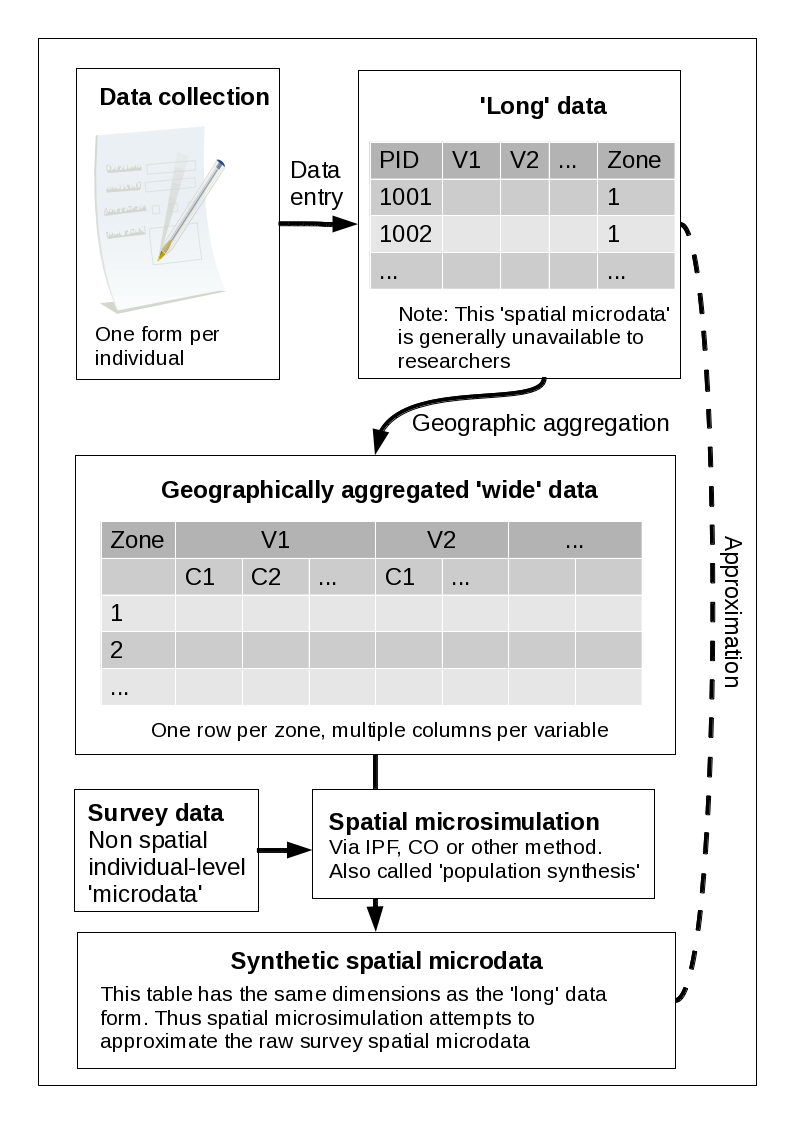
\includegraphics[width=10cm]{msim-schema}
\end{center}

\caption{Schema of iterative proportional fitting (IPF) and combinatorial optimisation
in the wider context of the availability of different data formats and spatial microsimulation. \label{fmsim-schema}}
\end{figure}

\subsection{What is IPF and why use it?} 
\label{swhatis}

In abstract terms, IPF is a procedure for assigning values to \emph{internal cells}
based on known marginal totals in a multidimensional matrix \citep{Cleave1995}.
More practically, this enables the calculation of the
\emph{maximum likelihood} estimate of the presence of
given individuals in specific zones.
Some confusion surrounds the procedure because it has multiple names:
the `RAS algorithm', `biproportional fitting' and to a lesser extent
`raking' have all been used to describe the procedure
at different times and in different branches of academic research \citep{Lahr2004}.
`Entropy maximisation' is a related technique, of which IPF is considered to be a
subset \citep{Johnston1993,Rich2012}.\footnote{As an
aside, IPF is considered by \citet{Rich2012} to be a particular
efficient for of entropy maximisation: ``The popularity of the IPF is therefore mainly due to the fact that it provides a
solution which is equivalent to that of the ME [maximum entropy]
approaches, but attained in a much more
computationally efficient way'' (p.~469).
}
Usage characteristics of these different terms are summarised in \cref{tterms}.

\begin{table}[htbp]
\caption{Usage characteristics of different terms for the IPF procedure, from the Scopus database.
The percentages refer to the proportion of each search term used to refer to IPF in different
subsets of the database: articles published since 2010 and mentioning ``regional'', respectively.}

\begin{center}
\begin{tabular}{lp{1.5cm}p{2.5cm}p{1.5cm}p{2.5cm}}
\toprule
Search term & N. citations & Commonest subject area & \% since 2010 & \% mentioning ``regional'' \\
\midrule
Entropy maximisation & 564 & Engineering & 30 & 9 \\
``Iterative proportional fitting''  & 135 & Mathematics & 22\ & 16 \\
``RAS Algorithm'' & 25 & Comp. science & 24 & 24 \\
``Iterative proportional scaling'' & 15 & Mathematics & 27 & 0 \\
Matrix raking & 12 & Engineering & 50 & 0 \\
Biproportional estimation & 12 & Social sciences & 17 & 33 \\
\bottomrule
\end{tabular}
\end{center}
\label{tterms}
\end{table}

Ambiguity in terminology surrounding the procedure has existed for a long time:
when Michael Bacharach began using the term `biproportional' late 1960s, he did so with the
following caveat: ``The `biproportional' terminology is not introduced in what
would certainly be a futile attempt to dislodge `RAS', but to help to abstract the
mathematical characteristics from the economic associations of the model'' \citep{bacharach1970biproportional}.
The original formulation of the procedure is generally ascribed to \citet{Deming1940},
who presented an iterative procedure for solving the problem of how to modify internal cell counts
of census data in `wide' form, based on new marginal totals. Without repeating
the rather involved mathematics of this discovery, it is worth quoting again from
\citet{bacharach1970biproportional}, who provided as clear a description as any of the procedure
in plain English: ``The method that Deming and Stephan suggested for
computing a solution was to fit rows to the known row sums and columns to the known
column sums by alternate [iterative] scalar multiplications of rows and columns of the
base matrix'' (p.~4). The main purpose for revisiting and further developing the technique
from Bacharach's perspective was to provide forecasts of the sectoral disaggregation of
economic growth models. It was not until later
(e.g.~\citealp{Holm1987}) that the procedure was rediscovered for geographic research.

Thus IPF is a general purpose tool with multiple uses. In this paper we focus on its
ability to \emph{disaggregate} the geographically aggregated data typically
provided by national statistical agencies to synthesise \emph{spatial microdata},
as illustrated in \cref{fmsim-schema}.
% But why would one want do this in the first place? % removed by db - can re-add for waffle!
% 
% % Each row in this aggregated form can 
% % represent the entire dataset or subsets thereof. (Geographical aggregation – one row 
% % per zone – is the most common form of aggregation, but any subsets, from social class, 
% % time period or other \emph{cross-tablulations} of the dataset can be used).
% 
% To answer this question, let us briefly consider the advantages and drawbacks of
% the ubiquitous wide data format, mentioned in the previous section.
% The main advantages of wide datasets are that
% they can summarise information about very many individuals
% in a relatively few rows, saving storage space, easing the analysis and
% % , critically for policy makers, % removed thanks to DB
% ensuring the anonymity of
% survey respondents. But the process of aggregation
% and associated information loss
% leads to the following disadvantages:
% \begin{itemize}
%  \item \emph{Binning of continuous variables:} we do
% not know from a wide dataset if the aforementioned person earning \pounds13,000 is in fact on a salary of
% \pounds10,000, \pounds15,000 or 
% anywhere in between
%  \item \emph{Loss of geographical resolution:} when aggregation is undertaken by geographical zones
% %  --- as is usually the case ---
%  spatial information is lost. Instead of knowing a person's precise home location, from the full dataset, we
% may only be able to pin them down to a relatively large administrative area.
%  \item \emph{Loss of cross-tabulation}: during the process of
% aggregation the links between different variables, often expressed as `contingency tables',
% is usually lost. For example a female cyclist may be represented as additional units in the
% ``cyclist'' and ``female'' categories, without knowledge of their interrelation.
% \end{itemize}
% % make bullet points???

In the \emph{physical sciences} both data formats are common and the
original long dataset is generally available. In the social sciences, by contrast, the long format is often unavailable
due to the long history of confidentiality
issues surrounding officially collected survey data.
It is worth emphasising that National Census datasets --- in which characteristics of 
every individual living in a state are recorded and which constitute some of the best datasets in social science ---
are usually only available
in wide form. This poses major challenges to researchers in the sciences who are
interested in intra-zone variability at the local level \citep{Whitworth2012,Lee2009}.

A related long-standing research problem especially prevalent in geography and regional science
is the scale of analysis. There is often a trade-off between the quality and resolution 
of the data, which can result in a compromise between detail and accuracy of results 
\citep{ballas2003microsimulation-30-years}. Often, researchers investigating 
spatial phenomena at many scales must use two datasets: one long non-spatial
survey table where each row represents the characteristics of an individual --- such as
age, sex, employment status and income --- and another wide, geographically aggregated 
dataset. IPF solves this problem when used in
spatial microsimulation by proportionally assigning individuals to zones of which they
are most representative.
% It is these `linking variables'
% that enable IPF to converge on the weights that best represent how representative each individual is
% of each zone, as described in the next section.

% could take this out...
% As illustrated in \cref{fmsim-schema}, wide datasets are
% are wider and shorter, containing multiple columns for each variable from the raw dataset,
% causing loss of information about the linkages between different variables, their \emph{cross tabulations}.
% The solution to this problem, however, makes the wide datasets even more unwieldy, as
% each new cross-tabulated variable adds $nv \times ncol(X)$  \emph{more} columns to the 
% wide dataset, where $nv$ is the number discrete categories in the new variable and $ncol(x)$
% is the existing number of columns in the wide data 
% table.\footnote{To 
% provide a concrete example, a cross-tabulation 
% of mode of travel to work by sex and social class would contain 540 (12 * 3 * 15) columns,
% due to the number of categories present in each variable. 
% Given that there are dozen of additional variables in any large census, this clearly becomes
% rapidly unwieldy as more variables are added.
% } % figure???
% The lack of cross tabulation is problematic because 
% in many cases information about the linkages between different variables is needed to 
% address policy-relevant questions. To pick one example related to 
% policies targeted at skilled unemployed young adults: how many unemployed people 
% reside in each geographical area who at the same time have a university degree, 
% are female and over 25 years old? This question is impossible to answer with a 
% geographically aggregated (wide) dataset.

\subsection{IPF in spatial microsimulation}
Spatial microsimulation tackles the aforementioned problems associated
with the prevalent geographically aggregated wide data form by simulating
the individuals within each administrative zone. The most detailed output of this process of 
spatial microsimulation is \emph{synthetic spatial microdata}, a long table of individuals with 
associated attributes and weights for each zone (see \cref{t:w} %???really
 for a simple example). 
Because these individuals correspond to observations in the survey dataset,
the spatial microdata generated in this way, of any size and complexity,
can be stored with only three columns: person identification number (ID),
zone and weight. Weights are critical to spatial microdata generated in this way, as they 
determine how representative each individual is of each zone.
Synthetic spatial microdata taken from a single dataset can therefore be
stored in a more compact way: a `weight matrix' is a matrix with rows representing
individuals and columns geographic zones. The internal cells reflect how reflective each
individual is of each zone.
% the same dataset can be stored using only two variables:  
% small area microdata 
% by combining the small area data with national survey data. The result of this process 
% of population synthesis (in its long % have we already defined long?
%  form --- it can also be represented in a wide table of counts)
%  is a table in which rows represent each 
% individual in the study region, with an additional column indicating the area of residence (Table 1).

Representing the data in this form offers a number of advantages
(Clarke and Holm, 1987). These include:
\begin{itemize}
 \item The ability to investigate intra-zone variation (variation within each zone can be analysed
 by sub-setting a single area from the data frame).
\item Cross-tabulations can be created for any combination of variables (e.g. age and employment status).
\item The presentation of continuous variables such as income as real numbers, 
rather than as categorical count data, in which there is always data loss.
\item The data is in a form that is ready to be passed into an individual-level model.
For example individual behaviour could simulate traffic, migration or the geographical distribution of future demand for healthcare.
\end{itemize}

% A potential downside of spatial microdata is that it can provide a misleading impression about the 
% quality and detail of the input data. It is important to remember that spatial microdata generated 
% in this way through spatial microsimulation are only as good as the constraint variables and the 
% extent to which the national dataset is representative of the zones in the study area.

These benefits have not gone unnoticed by the spatial modelling community.
Spatial microsimulation is now considered by some to be more than a methodology:
it can be considered as a research field in its
own right, with a growing body of literature, methods and software tools \citep{Tanton2013}.
In tandem with these methodological developments, a growing number of applied studies
take advantage of the possibilities opened up by spatial microdata.
Applications are diverse, including studies on:
% Papers that have used IPF in this context (or a substitutable method such as simulated annealing)
% have explored a range of regional economic problems that purely aggregate level analyses struggle to address.
% These include:
\begin{itemize}
 \item The individual and local impacts
of job losses and gains from the closure \citep{Ballas2006}
or opening \citep{VanLeeuwen2010} of new businesses.
\item Inequalities between individuals and zones in educational opportunities
and attainment \citep{Kavroudakis2012}.
\item Commuting patterns and the distributional impacts
of new transport policies \citep{Lovelace2014-jtg}.
\item The spatial behavior of farmers and rural residents
\citep{Hynes2009,van2013determinants}.
\item Investigation of the local impacts of economic development
in the marine energy sector \citep{Morrissey2013a}.
\item The socio-spatial impacts of changes in taxation policy \citep{campbell2013spatial}.
\item The optimal location of health services based
on estimates of individual level behaviour and obesity rates \citep{Tomintz2008,Clarke2010-valid}.
\item The use of spatial microsimulation in combination with
agent based models to simulated student populations \citep{Wu2010},
estimate the energy impacts of freight transport \citep{Zuo2013a}
and to estimate the impacts of urban regeneration \citep{jordan2011agent}.
\end{itemize}

Various strategies for generating the synthetic spatial microdata used
in such studies are available,
as described in recent overviews on the subject
\citep{Tanton2013, Ballas2013-4policy-analysis, Hermes2012a}.
However, it is not always clear which is most appropriate in different situations.
There has been work testing % \citep{Jirousek1995}
and improving model results \citep{teh2003improving}, yet research focused on
systematically and transparently testing
the underlying algorithms for generating synthetic spatial microdata is
limited \citep{harland2012}.
This research gap, addressed in this paper, is highlighted 
in the conclusions of a recent Reference Guide to spatial microsimulation
\citep[p~270]{Clarke2013-concs}:
``It would be desirable if the spatial microsimulation community were able to continue to
analyse which of the various reweighting/synthetic reconstruction techniques is most accurate
--- or to identify whether one approach is superior for some applications while another
approach is to be preferred for other applications''.
% Before proceeding to the model experiments, we
% provide a brief overview of the applications of IPF in regional science
% and outline the theory underlying the procedure based on a simple example. 
% The longest-established and most straight-forward of
% these is Iterative Proportional Fitting (IPF), the performance of which is the subject of this paper...

% \subsection{Applications}
% \textbf{Dimitris and Eveline: please fill in this section}
% Applications of IPF include using it ...

% The application of greatest interest to social scientists, and others working %!!! re-include
% with `ecological' data \citep{Openshaw1984}, is as a method of
% generating spatial microdata: individual level data allocated to zones.
%  IPF enables the generation
% individual level data allocated to specific zones: the creation of
% \emph{spatial microdata}.

% \section{IPF: theory and a worked example}
% Iterative Proportional Fitting has a long history in Statistics and the social
% sciences (especially in Economics and Geography).
% In statistical language, IPF is used to estimate the values of internal
% cells in a cross-tabulated table to fit known margins.
% The method is also known as matrix raking or scaling,
% biproportional fitting, RAS, and entropy maximising.
% There are a number of texts discussing the method in a mathematical formal
% way in some detail (for example \citealp{Mosteller1968, Fienberg1970, Pritchard2012}).
% \citep{Birkin1988} provide a succinct presentation of the
% mathematics of IPF and their work is the foundation of
% the work presented here...% described in origin; rethink this...???
% 
\section{The IPF algorithm: a worked example} \label{s:theory}
In most modelling texts there is a precedence of theory over
application: the latter usually flows from the former
(e.g.~\citealp{batty1976urban}).  
As outlined in \cref{swhatis}, however, the theory underlying IPF has
been thoroughly demonstrated in research stemming back to the 1940s.
\emph{Practical} demonstrations
% , focused on making the algorithm as accessible as possible to others,
are comparatively rare.

% This section presents a
% simple worked example. The steps are presented in detail
% to allow readers to follow the method, address the theory:practice balance and
% ensure accessibility to understanding of the method.

That is not to say that reproducibility is completely absent in the field.
\citet{Simpson2005} and \citet{Norman1999a}
exemplify their work with code snippets from an implementation
of IPF in the proprietary software SPSS and reference to
an Excel macro that is available on request, respectively.
\citet{Williamson2007} also represents
good practice, with a manual for running 
combinatorial optimisation algorithms described in previous work.
\citet{Ballas2005c} demonstrate IPF with a worked example
to be calculated using mental arithmetic, but do not progress to
illustrate how the examples are then implemented in computer code.
This section builds on and extends this work, by first outlining an example that
can be completed using mental arithmetic alone before illustrating its
implementation in code. A comprehensive introduction to
% the basic theory and practicalities of implementing IPF in R for spatial microsimulation
this topic is provided in a tutorial entitled
 ``Introducing spatial microsimulation with R: a practical'' \citep{lovelace2014introducing}. This section builds on the tutorial by providing
context and a higher level description of the process.
 % Have you implemented in R???

% Importantly for for reproducible research this theory section
% is illustrated with a simple worked example that culminates in
% a question to the reader, to test his or her understanding.

% It is worth restating that IPF is a simple statistical procedure, % why???
% ``in which cell counts in a contingency
% table containing the sample observations are scaled to be consistent with
% various externally given population marginals'' \citep{mcfadden2006testing}. In
% other words, and in the context of \emph{spatial} microsimulation, IPF produces
% maximum likelihood estimates for the frequency with which people appear in
% different areas.

% The method is also known as `matrix raking' or the RAS %%% may want to re-include at some point
% algorithm, 
% % (\citealp{Birkin1988, Muller2010,Simpson2005, Kalantari2008, Jirousek1995})
%  and has been described as one
% particular instance of a more general procedure of `entropy maximisation'
% \citep{Johnston1993, blien1998entropy}.
% The mathematical properties of IPF
% have been described in several papers
% (\citealp{Bishop1975, Fienberg1970, Birkin1988}).
% Illustrative examples of the procedure can be found in
% \citet{Saito1992}, \citet{Wong1992}
% and \citet{Norman1999a}. \citet{Wong1992} investigated the reliability of IPF
% and evaluated the importance of different factors influencing the its
% performance. Similar methodologies have since been employed by
% \citet{Mitchell2000}, \citet{Williamson2002} and
% Ballas et al.~\citeyearpar{Ballas2005c}
% to investigate a wide range of phenomena.

% The example described below is a modified version
% \citet{Ballas2005c}.\footnote{In \citet{Ballas2005c}
% the interaction between the age and sex constraints are assumed to be known.
% (Their equivalent of \cref{t:s2} contains data for every cell,
% not question marks.) This results in IPF converging instantly.
% However, in Census data, such cross-tabulation is
% often absent, and IPF must converge over multiple constraints and
% iterations. This latter scenario is assumed in the worked example below. Other
% worked examples of the principles are provided in \citet[Appendix
% 3]{johnston1985geography} (for entropy maximisation), \citet{Norman1999a} and
% \citet{Simpson2005} (using the proprietary statistical software SPSS).
% }
We begin with some hypothetical data.
Table \ref{t:w}  describes a
hypothetical microdataset comprising 5 individuals, who are defined by two
constraint variables, age and sex. 
Table \ref{t:s} contains aggregated data
for a hypothetical area, as it might be downloaded from census dissemination
portals such as Casweb.\footnote{Casweb
    (\href{http://casweb.mimas.ac.uk/}{casweb.mimas.ac.uk/})
is an online portal for academics and other researchers to
gain access to the UK's official census data in geographically
aggregated form.} \Cref{t:s2} illustrates this table in a different form,
demonstrating the unknown links between age and sex. The job of the IPF
algorithm is to establish estimates for the unknown cells, which are
optimized to be consistent with the known row and column marginals.

\begin{table}[!h]
\centering
\caption[A hypothetical input microdata set]{A
hypothetical input microdata set (the original
weights set to one). The bold value is used subsequently for
illustrative purposes.}
\begin{center}
\begin{tabular}{llll}
\toprule
{Individual } & {Sex} & {Age} & {Weight} \\
\midrule
1 & Male & 59 & 1 \\
2 & Male & 54 & 1 \\
3 & {Male} & {35} & \textbf{1} \\
4 & Female & 73 & 1 \\
5 & Female & 49 & 1 \\
% 1 & 59 & m \\
% 2 & 54 & m \\
% 3 & 35 & m \\
% 4 & 73 & f \\
% 5 & 49 & f \\
\bottomrule
\end{tabular}
\end{center}
\label{t:w}
\end{table}
\vspace{1cm}


\begin{table}[!htbp]
\caption{Hypothetical small area constraints data ($s$).}
\begin{center}
\begin{tabular}{cllll}
\toprule
Constraint $\Rightarrow$ & \multicolumn{2}{c}{$i$}& \multicolumn{2}{c}{$j$}\\
Category $\Rightarrow$ & $i_1$ & $i_2$ & $j_1$ & $j_2$ \\
Area $\Downarrow$  & Under-50 & Over-50 &  Male & Female\\
1  & 8 & 4 & 6 & 6\\
\bottomrule
\end{tabular}
\end{center}
\label{t:s}
\end{table}
\vspace{1cm}

\begin{table}[!htbp]
\caption[Small area constraints expressed as marginal totals]{Small
area constraints expressed as marginal totals, and the cell
values to be estimated.}
\begin{center}
\begin{tabular}{cllll}\toprule
Marginal totals&  & \multicolumn{2}{c}{$j$} & \\
& Age/sex & Male & Female & T\\ \midrule
\multirow{2}{*}{$i$} & Under-50 & \textbf{?} & ? & 8\\
& Over-50 & ? & ? &4 \\
& T & 6 & 6 &12\\
\bottomrule
\end{tabular}
\label{t:s2}
\end{center}
\end{table}

\FloatBarrier

Table \ref{t:m} presents the
hypothetical microdata in aggregated form,
that can be compared directly to Table \ref{t:s2}.
Note that the integer variable age has been converted into
a categorical variable in this step, a key stage in geographical aggregation.
Using these data it is possible to readjust the weights of the hypothetical
individuals, so that their sum adds up to the totals given in Table
\ref{t:s2} (12). In particular, the weights can be readjusted by multiplying them by
the marginal totals, originally taken from
Table \ref{t:s} and then divided by the respective marginal total in \ref{t:m}.
Because the total for each small-area constraint is 12, this must be
done one constraint at a time. This
is expressed, for a given area and a given constraint ($i$, age in this case)
in \cref{eq:ipf}.

\begin{table}[!htbp]
\caption[The aggregated results of the weighted
microdata set]{Aggregated results of the weighted
microdata set ($m(1)$).
Note, these values depend on the
weights allocated in Table \ref{t:w} and therefore
 change after each iteration.}
\begin{center}
\begin{tabular}{cllll}\toprule
Marginal totals&  & \multicolumn{2}{c}{$j$} & \\
& Age/sex & Male & Female & T\\ \midrule
\multirow{2}{*}{$i$} & Under-50 & \textbf{1} & 1 & 2\\
& Over-50 & 2 & 1 &3 \\
& T & 3 & 2 &5\\
\bottomrule
\end{tabular}
\end{center}
\label{t:m}
\end{table}

\begin{equation}
w(n+1)_{ij} = \frac{w(n)_{ij} \times sT_{i}}{mT(n)_{i}}
\label{eq:ipf}
\end{equation}

In \cref{eq:ipf}, $w(n+1)_{ij}$ is the new weight for individuals with characteristics $i$
(age, in this case), and $j$ (sex),  $w(n)_{ij}$ is the original
weight for individuals with these characteristics, $sT_{i}$ is element
marginal total of the small area constraint, $s$
(Table \ref{t:s}) and $mT(n)_{i}$ is the marginal total of category
$j$ of the aggregated results of the weighted
microdata, $m$ (Table \ref{t:m}). $n$ represents the iteration number.
Although the marginal totals of $s$ are known, its cell values
are unknown. Thus, IPF estimates the interaction (or cross-tabulation)
between constraint variables.
Follow the emboldened values in the Tables \ref{t:w} to \ref{t:new-weights}
to see how the new weight of individual 3 is calculated for the sex constraint.
Table \ref{t:new-weights} illustrates the weights that result. Notice that the
sum of the weights is equal to the total population, from the constraint variables.

\begin{table}[htbp]
\caption{Reweighting the hypothetical microdataset in order to fit
Table \ref{t:s}.}

\begin{center}
\begin{tabular}{lllll}
\toprule
{Individual} & {Sex} & {age-group} & {Weight} &
{New weight, w(2)} \\ \midrule
1 & Male & Over-50 & 1 & $1 \times 4/3 = \frac{4}{3}$ \\
2 & Male & Over-50 & 1 & $1 \times 4/3 = \frac{4}{3}$ \\
3 & Male & Under-50 & 1 & $\textbf{1} \times
\textbf{8}/\textbf{2} = 4$ \\
4 & Female & Over-50 & 1 & $1 \times 4/3 = \frac{4}{3}$ \\
5 & Female & Under-50 & 1 & $1 \times 8/2 = 4$ \\
\bottomrule
\end{tabular}
\end{center}
\label{t:new-weights}
\end{table}

\FloatBarrier

After the individual level data have been re-aggregated (\cref{t:m2}),
the next stage is to repeat \cref{eq:ipf} for the age constraint to generate a
third set of weights, by replacing
the $i$ in $sT_{i}$ and $mT(n)_{i}$ with $j$ and incrementing the value of n:

\begin{equation}
w(3)_{ij} = \frac{w(2)_{ij} \times sT_{j}}{mT(2)_{j}}
\label{eq:ipf2}
\end{equation}

Apply \cref{eq:ipf2} to the information above and that presented in \cref{t:m2}
results in the following vector of new weights, for individuals 1 to 5:
\begin{equation}
%  w(3) = (\frac{6}{5}, \frac{?}{?}, \frac{18}{5}, \frac{?}{?}, \frac{9}{2})
  w(3) = (\frac{6}{5}, \frac{6}{5}, \frac{18}{5}, \frac{3}{2}, \frac{9}{2})
\end{equation}

\FloatBarrier

As before, the sum of the weights is equal to the population of the area (12).
Notice also that after each iteration the fit between the marginal
totals of $m$ and $s$
improves. The total absolute error (TAE, described in the next section)
improves in $m(1)$ to $m(2)$ from
14 to 6 in \cref{t:m} and \cref{t:m2} above. TAE for $m(3)$ (not shown,
but calculated by aggregating $w(3)$) improves even more, to 1.3.
This number would eventually converge to 0 through subsequent
iterations, as there are no empty cells in the input microdataset,
a defining feature of IPF (see \cref{smempty} for more on the impact of empty cells).

\begin{table}[htbp]
\centering
\caption[Aggregated results after constraining for age]{The
aggregated results of the weighted
microdata set after constraining for age ($m(2)$).
}

\begin{tabular}{cllll}\toprule
Marginal totals&  & \multicolumn{2}{c}{$i$} & \\
& Age/sex & Male & Female & T\\ \midrule
\multirow{2}{*}{$j$} & Under-50 & 4 & 4 & 8\\
& Over-50 & $\frac{8}{3}$ & $\frac{4}{3}$ & 4 \\
& T & $6\frac{2}{3}$ & 5$\frac{1}{3}$ & 12\\
\bottomrule
\end{tabular}
\label{t:m2}
\end{table}

The above process, when applied to more categories (e.g.~socio-economic class)
and repeated iteratively until a satisfactory convergence occurs, results in a
series of weighted microdatasets, one for each of the small areas being
simulated. This allows for the estimation of variables whose values are not
known at the local level (e.g.~income) \citep{Ballas2005c}. An issue
with the results of IPF
is that it results in non-integer weights: fractions of individuals
appear in simulated areas. This is not ideal
for certain applications, leading to the development of strategies
to 'integerise' the fractional weights illustrated in \cref{t:m2}.
Methods for performing integerisation are discussed in
\citep{Ballas2005c}, \citep{Pritchard2012} and, most recently
in \citep{Lovelace2013-trs}, who
systematically benchmarked and compare different procedures.
It was found that the `truncate, replicate, sample' (TRS)
and `proportional probabilities' methods were most accurate.
These methods are therefore used to test the impact of
integerisation in this paper.
% Based on this last paper, we use the TRS methodology to explore the impacts
% of integerisation in this paper.
% Integer weights allow the results of spatial
% microsimulation to be further processed using dynamic microsimulation and agent
% based modelling techniques.

% A key benefit from a policy perspective is that
% IPF and other spatial microsimultion techniques
% can provide estimation of variables whose values are not
% known at the local level (e.g. income).
% Spatial microsimulation can also provide insight into the likely
% distribution of individual level variables about which only
% geographically aggregated statistics have been made available.
% An issue
% with the results of IPF (absent from combinatorial optimisation methods),
% however, is that it results in non-integer weights: fractions of individuals
% appear in simulated areas.

% \subsection{Implementing IPF in R} \label{simplementing}
% The above example is best undertaken by hand, probably with a pen and paper
% to gain an understanding of IPF, before the process is automated for 
% larger datasets. This section explains how the IPF
% algorithm described above can be implemented in R.
% This section is based on ``Spatial microsimulation in R: a
% beginner’s guide to iterative proportional fitting (IPF)'', a tutorial
% written to accompany a methods paper on integerisation
% \citep{Lovelace2013-trs}.

% \footnote{This 
% tutorial is available from Rpubs, a site dedicated
% to publishing R analyses that are reproducible. It uses the RMarkdown
% mark-up language, which enables R code to be run and presented within
% documents. See http://rpubs.com/RobinLovelace/5089 \label{fnrpub} .
% }

\section{Evaluation techniques}
% Add correlation matrix at end of links between these
% Really should write a paper on this to update Voas2001 - not the place here
To verify the integrity of any model, it is necessary to compare its outputs
with empirical observations or prior expectations gleaned from theory.
The same principles apply to spatial microsimulation, which can be evaluated using
both \emph{internal} and \emph{external} validation methods \citep{Edwards2009}.
\emph{Internal validation} is the process whereby
the aggregate-level outputs of spatial microsimulation are compared with
the input constraint variables. It is important to think carefully about
evaluation metrics because results can vary depending on the measure used
\citep{Voas2001}.

Internal validation typically tackles such issues
as ``do the simulated populations in each area
microdata match the total populations implied by the constrain variables?''
and ``what is the level of correspondence between the cell values of different
attributes in the aggregate input data and the aggregated results of spatial microsimulation?''
A related concept from the agent based modelling literature is
\emph{verification}, which asks the more general question,
``does the model
do what we think it is supposed to do?'' \citep[p.~131]{ormerod2009validation} 
% Ideally we would hope for a perfect fit between the input
% and output datasets during internal evaluation.
\emph{External validation} is the process whereby the variables that are
being estimated are compared to data from another source,
external to the estimation process, so the output dataset is compared with
another known dataset for those variables.
Both validation techniques are important in modelling exercises for reproducibility and to ensure critical advice is not made
based on coding errors \citep{ormerod2009validation}.
%... ?

For dynamic microsimulation scenarios,
calculating the sampling variance (the variance
in a certain statistic, usually the mean, across multiple samples)
across multiple model runs
is recommended to test if differences between different
scenarios are statistically significant \citep{goedeme2013testing}.
In static spatial
microsimulation, sub-sampling
from the individual level dataset or running stochastic processes
many times are ways to generate such statistics for tests
of significance. Yet these statistics will only apply to a small part
of the modelling process and are unlikely to relate to
the validity of the process overall \citep{Lovelace2013-trs}.

This section briefly outlines the evaluation techniques
used in this study for \emph{internal validation}
of static spatial microsimulation models.
% , in addition to a new implementation of
% the S\o rensen-Dice coefficient for continuous variables. % Just making more work!!!
The options for external
validation are heavily context dependent so should be decided on a
case-by-case basis.
External validation is thus mentioned in the discussion,
with a focus on general principles
rather than specific advice. The three quantitative
methods used in this study (and the visual method of scatter plots)
are presented in ascending order of complexity
and roughly descending order of frequency of use, ranging from 
the coefficient of determination ($R^2$) through total and standardised
absolute error ($TAE$ and $SAE$, respectively)
% to the proportion of values deviating from the expected
% value by a predefined amount ($P > 0.5$). The preferred metric
to root mean squared error (RMSE).
This latter option is our preferred metric, as described below.
% The equations for each metric can be found in the associated references.

Before these methods are described, it is
worth stating that the purpose is not to find the `best' evaluation metric:
each has advantages and disadvantages, the importance of which will vary depending on the
nature of the research. The use of a variety of techniques in this paper
is of interest in itself. The high degree of correspondence between them (presented in \cref{cresults}),
suggests that researchers need only to present one or two metrics (but should
try more, for corroboration)
to establish relative levels of goodness of fit between
different model configurations.

The problem of internal validation
(described as `evaluating model fit') was tackled in detail by \citet{Voas2001}.
Chi-squared, Z-scores, absolute error and entropy-based methods
were tested, with no clear `winner' other than the advocacy of
methods that are robust, fast and easy to understand (standardized absolute
error measures match these criteria well).
The selection of evaluation methods is determined by
the nature of available data:
``Precisely because a full set of raw census data is not
available to us, we are obliged to evaluate our simulated populations by comparing
a number of aggregated tables derived from the synthetic data set with published
census small-area statistics'' \citep[p.~178]{Voas2001}.
A remaining issue is that the results of many evaluation metrics vary depending
on the areal units used, hence advocacy of `scale free' metrics \citep{Malleson2012}	.

% \subsection{Descriptive statistics}
% 
% Useful basic statistics to describe and compare datasets are 
% the mean, median and standard deviation of cell counts in the
% simulated and known aggregate-level database.
% These are useful `sanity checks': if the mean population across all zones or
% for a particular constraint differs greatly from expectations, there is clearly
% a problem. These summary statistics are dependent on the
% size of the dataset. To compare datasets of widely varying populations,
% dimensionless statistics can be used.
% The coefficient of variation, the ratio of the standard deviation to the mean is
% an example of a dimensionless statistic robust to population size.
 

\subsection{Scatter plots}
A scatter plot of cell counts for each category for the original and simulated variables is
a basic but very useful preliminary diagnostic tool in spatial microsimulation
\citep{Ballas2005c,Edwards2009}.
In addition, marking the points, depending on the
variable and category % have these been defined?
which they represent, can help identify which variables are particularly problematic,
aiding the process of improving faulty code (sometimes referred to as `debugging').

In these scatter plots each data point represents a single zone-category
combination (e.g.~16-25 year old female in zone 001), with the x axis value corresponding
to the number of individuals of that description in the input constraint table.
The y value corresponds to the
aggregated count of individuals in the same category in the aggregated
(wide) representation of the spatial microdata output from the model. % have we defined spatial microdata?
This stage can be undertaken either before or after \emph{integerisation}
(more on this below). As taught in basic statistics courses, the closer the points to the
1:1 (45 degree, assuming the axes have the same scale) line, the better the fit.

\subsection{The coefficient of determination}
The coefficient of determination (henceforth $R^2$) is the 
square of the Pearson correlation coefficient for describing the
extent to which one continuous variable explains another.
$R^2$ is a quantitative
indicator of how much deviation there is from this ideal
1:1 line. It varies from 0 to 1,
and in this context reveals how closely the 
simulated values fit the actual (census) data.
An $R^2$ value of 1 represents a perfect fit; an $R^2$ value
close to zero suggests no correspondence
between then constraints and simulated outputs (i.e. that the model has failed).
We would expect to see $R^2$ values approaching 1 for
internal validation (the constraint) and a strong
positive correlation between target variables that have been estimated and
external datasets (e.g. income). A major limitation of $R^2$ is that
it takes no account of \emph{additive} or \emph{proportional} differences
between estimated and observed values, meaning that it ignores systematic
bias (see \citealp{Legates1999GOF} for detail).
This limitation is less relevant for spatial microsimulation results
because they are generally population-constrained. 

% A potential disadvantage of $R^2$ is that it provides no
% information about the formula linking simulated data to the 
% known constraints: it expresses absolute Rather, $R^2$ expresses the fit of the data to the ‘best fit’ line through that data. That is, the coefficient of determination is providing information about precision, not accuracy (Edwards and Tanton, 2013).

% One way to do this is with a t test. With a spatial microsimulation model validation, the data are paired (given we are comparing simulated with actual data), thus an equal variance 2-tailed t test can be used to determine if there is any significant difference between the two datasets (i.e. simulated and actual). Thus, if the simulation is robust, we would expect to see no significant differences between the simulated and actual values for the input variables (and estimated/output variables, if known data are available). This enables the model accuracy to be assessed, as opposed to simply its precision.

% \subsection{Standard error around identity (SEI)}
% here SEI is the standard error around identity, y are the estimated values for
% each area, y rel are the reliable estimates for each area from a census or other
% data source and y rel is the mean estimate for all areas where reliable data are available.
% This estimate has been used in validation by both Ballas and Tanton (see Ballas et al. 2007; Tanton et al. 2011).

\subsection{Total Absolute and Standardized Error (TAE and SAE)}
Total absolute error (TAE) is the sum of the absolute (always positive)
discrepancies between the simulated
and known population in each cell of the geographically aggregated (wide format)
results. The standardised absolute error (SAE) is
simply TAE divided by the total population \citep{Voas2001}.
TAE provides no level of significance, so thresholds are used.
\citet{clarke2001regional} used an error threshold of 80 per cent of the
areas with less than 20 per cent error (SAE \textless 0.20);
an error threshold of 10\%  (SAE \textless 0.1) can also been used % check!!!
\citet{smith2007simhealth}. % really??? probably
Due to its widespread use, simplicity and scale-free nature,
SAE is an often preferred metric.

% \subsection{The modified Z-score}
% The Z-statistic is a commonly
% used measure, reporting the number of standard deviations
% a value is from the mean.
% In this work we report $zm$, a modified version to the Z-score
% metric that is robust to very small expected cell values
% \citep{Williamson1998}.
% Z-scores apply to individual cells (for a single constraint in a single area).
% and also provide a global statistic on model fit ($Zm$), defined
% as the sum of all $zm^2$ values \citep{Voas2001}.
% The measure of
% fit has the advantage of taking into account absolute, rather than just
% relative, differences between simulated and observed cell count:
% \begin{equation}
%  Zm_{ij} = (r_{ij} - p_{ij}) \Bigg/ \left(\frac{p_{ij}(1 -
% p_{ij}))}{\sum\limits_{ij}U_{ij}}\right)^{1/2}
% \end{equation}
% 
% where
% 
% \begin{center}
% \begin{math}
%   p_{ij} = \frac{U_{ij}}{\sum\limits_{ij}U_{ij}} \qquad and \qquad r_{ij} =
% \frac{T_{ij}}{\sum\limits_{ij}U_{ij}}
% \end{math}
% \end{center}
% 
% To use the modified Z-statistic as a measure of overall model fit, one simply
% sums the squares of $zm$ to calculate $Z{m}^{2}$. This measure can handle
% observed cell counts below 5, which chi-squared tests cannot \citep{Voas2001}.

% \subsection{Proportion of values deviating from expectations $E > 5\%$}
% The proportion of values which fall beyond 5\% of the actual values is a simple
% metric of the quality of the fit.
% It focusses on the proportion of values which are close to expected, rather than
% the overall fit, so is robust to outliers.
% The $E > 5\%$ metric implies that getting a perfect fit is not
% the aim, and penalises relationships that have a large number of moderate outliers,
% rather than a few very large outliers. The precise
% definition of 'outlier' is somewhat arbitrary (one could just as well use 1\%).

% Spatial indicators etc??? Add equations to above methods soooon

\subsection{Root mean square error}
Root mean square error (RMSE) and to a lesser extent mean absolute error (MAE)
have been frequently
used in both social and physical sciences as a metric of model fit
\citep{Legates1999GOF,Ngo2012}. %!!! equations
Like SAE, the RMSE takes the
discrepancies between the simulated and known values, squares these and
divides the sum by the total number of observations (areas in our case), after
which the root is taken. The MAE basically does the same without the square and
root procedure.  The former has the benefit of being widely used and understood,
but is
influenced by the mean value in each zone. Recent research in climate model
evaluation suggests that the lesser known but simpler $MAE$ metric is preferable
to RMSE in many ways \citep{Willmott2005}.
% Therefore both metrics are presented in this paper.
We use the RMSE error in the final results as this is a widely understood and
applied method with a proven track record in the social sciences.

\section{Input data}
The size and complexity of input data have a strong
influence on the results of spatial microsimulation models.
Especially important are the
number of constraint variables and categories.
We wanted to test the method under a range of conditions.
Therefore, three unrelated scenarios, each with their own input datasets
were used. These are referred to as `simple', `small-area' and
`sheffield'. Each consists of a set of aggregate constraints and corresponding
individual-level survey tables.
To ensure reproducibility, all the input data (and code)
used to generate the results reported
in the paper are available online on the code-sharing site
GitHub.\footnote{The individual level survey tables
are anonymous and have been `scrambled' to enable their
publication online and can be downloaded by anyone from
http://tinyurl.com/lgw6zev
\href{http://tinyurl.com/lgw6zev}{tinyurl.com/lgw6zev}.
This enables the results to be replicated by others,
without breaching the user licenses of the data.}

The simplest scenario consists of 6 zones which must be populated by the
data presented in the previous section (see \cref{t:w}).
% sample survey dataset of only five individuals, constrained by two variables (age and sex).
This scenario is purely hypothetical and is used to represent the IPF procedure
and the tests in the simplest possible terms. Its small size allows the entirety
of the input data to be viewed in a couple of tables 
(see \cref{t:w} and \cref{t2}, the first row of which is used
to exemplify the method). As with all
data used in this paper, these tables can be
viewed and downloaded online.

% \begin{table}[htbp]
% \caption{Individual-level data for the simple scenario. The file, `vailable from
% the GitHub in the folder
% `\href{
% https://github.com/Robinlovelace/IPF-performance-testing/tree/master/input-data/
% small-area-eg}{input-data}'} % where???
% \begin{center}
% \begin{tabular}{rrl}
% \toprule
% \multicolumn{1}{l}{Id} & \multicolumn{1}{l}{Age} & Sex \\
% \midrule
% 1 & 59 & m \\
% 2 & 54 & m \\
% 3 & 35 & m \\
% 4 & 73 & f \\
% 5 & 49 & f \\
% \bottomrule
% \end{tabular}
% \end{center}
% \label{t1}
% \end{table}

\begin{table}[htbp]
\caption{Geographically aggregated constraint variables for the simple
scenario.}
\begin{center}
\begin{tabular}{rrrrr}
\toprule
\multicolumn{1}{l}{} & \multicolumn{2}{c}{Age constraint} & \multicolumn{2}{c}{Sex constraint} \\
\multicolumn{1}{l}{Zone} & \multicolumn{1}{c}{16--49} & \multicolumn{1}{c}{50+} & \multicolumn{1}{c}{m} & \multicolumn{1}{c}{f} \\
\midrule
1 & 8 & 4 & 6 & 6 \\
2 & 2 & 8 & 4 & 6 \\
3 & 7 & 4 & 3 & 8 \\
4 & 5 & 4 & 7 & 2 \\
5 & 7 & 3 & 6 & 4 \\
6 & 5 & 3 & 2 & 6 \\
\bottomrule
\end{tabular}
\end{center}
\label{t2}
\end{table}

The next smallest input dataset, and the most commonly used scenario in the paper, 
is `small-area'. The area constraints consist of 24 Output Areas (the smallest 
administrative unit in the UK), with an average adult population of 184.
Three constraint files describe the number of hours worked, the marital status and the
tenancy of these 
individuals (although tenancy in fact counts houses, not people): the files can
be accessed from `small-area-eg', within the `input-data' folder of the online
repository.\footnote{These datasets can be found in the `input-data'
sub-directory of the \href{http://tinyurl.com/lgw6zev}{Supplementary Information}.}
% Add these!!!
% A sample of these constraint variables is presented in \cref{t3} below. % aren't we putting ind. data 1st?
% 
% \begin{table}[htbp]
% \caption{Sample of constraint variables from the first 5 rows of the small-area-eg input dataset.}
% \begin{center}
% \begin{tabular}{rrrrr}
% \toprule
% \bottomrule
% \end{tabular}
% \end{center}
% \label{t3}
% \end{table}

The individual-level table that complements these geographically aggregated count constraints 
is taken from Understanding Society wave 1. These have been randomised to ensure anonymity
but they are still roughly representative of real data. The table consists of 1768 rows of 
data and is stored in R’s own space-efficient filetype (see ``ind.RData'', which must be opened in 
R).

% This individual level data consists of the same 3 % re-add this!!!
% constraint variables as provided in \cref{t3} in addition
% to one `target variable': monthly pre-tax income in pounds stirling. 

% \begin{table}[htbp]
% \caption{Randomly selected sample of 5 individuals taken from the individual-level dataset.}
% \begin{center}
% \begin{tabular}{rrrrr}
% \toprule
% \bottomrule
% \end{tabular}\	
% \end{center}
% \label{t4}
% \end{table}

% ... More here on loading-up this data.

\section{Method: model experiments}
\subsection{Baseline conditions} \label{smbase}
Using the three different datasets, the effects of five model settings were
assessed: number of constraints and iterations; initial weights; empty cell
procedures; and integerisation. In order to perform a wide range of
experiments, in which only one factor is altered at a time, 
baseline scenarios were created. These are model runs with sensible 
defaults and act as reference points against which alternative runs are compared.
The baseline scenarios consist of 3 iterations. In the `simple' scenario (with 2 constraints), 
there are 6 constraint-iteration permutations.
% \Cref{tblresults1} shows !!! removed as table 10 is absent!
The
fit improves with each step.\footnote{The exception is $p5$,
which reaches zero in the second iteration. $pcor$ continues to improve however, 
even though the printed value, to 6 decimal places, is
indistinguishable from 1 after two complete iterations.}

The main characteristics of the baseline model for each scenario area
presented in \cref{tbase}. The meaning of the
row names of \cref{tbase} should become clear throughout this section.

\begin{table}[htbp]
\caption{Characteristics of the baseline model run for each scenario.}
\begin{center}
\begin{tabular}{lrrr}
\toprule
Scenario & \multicolumn{1}{l}{Simple} & \multicolumn{1}{l}{Small area} & \multicolumn{1}{l}{Sheffield} \\
\midrule
N. constraints & 2 & 3 & 4 \\
N. zones & 6 & 24 & 71 \\
Av. individuals/zone & 10 & 184 & 3225 \\
Microdataset size & 5 & 1768 & 4933 \\
Average weight & 1.3 & 0.1 & 0.65 \\
\% empty cells & 0\% & 21\% & 85\% \\
\bottomrule
\end{tabular}
\label{tbase}
\end{center}
\end{table}


% The baseline `small-area' scenario consists of three
% iterations of IPF, in which all three constraints were
% used. 

\subsection{Constraints and iterations}
These were the simplest model experiments, requiring only
additional iterations and re-arrangement of the order
in which constraints were applied. 1, 3 and 10 iteration (up to 20 are
reported in the literature, but we found no difference in the
results beyond 10) are reported in the final
results.\footnote{For
an explanation of how to modify model parameters, see the `README.md' text
file in the \href{http://tinyurl.com/lgw6zev}{Supplementary Information}.}
% and `convergence graphs' were created to show how model % !!! really should add this after review!!! %TODO
% fit improved from one iteration-constraint combination to the next.
%
%To alter the number of iterations used in each model, one simply
%changes the number in the following line of code (the default is 3):
%
%\begin{lstlisting}
%num.its <- 3
%\end{lstlisting}
% 
%The code for running the constraints in a different order
%is saved in `etsim-reordered.R'.
%In this script file, the order in which constraints ran was systematically altered.
The order with the greatest impact on the results is the one reported
in the final results table (\cref{tsum}).

\subsection{Initial weights}
The impact of initial weights was tested in two ways: first, the impact
of changing a sample of one or more initial weight values by a set
amount was explored. Second, the impact of gradually increasing the size of the initial 
weights was tested, by running the same model experiment several times, 
but with incrementally larger initial weights applied to a pre-determined set of individuals.

In the simplest scenario, the
initial weight of a single individual was altered 
repeatedly, in a controlled manner.
%The code enabling this model experiment 
%is contained in the file `etsim-weights.R'. 
To observe the impacts of altering the weights in this way
the usual tests of model fit were conducted. In addition,
the capacity of initial weights to influence an individual's 
final weight/probability of selection was tested by tracing its
weight into the future after each successive constraint and iteration. 
This enabled plotting original vs simulated weights under a 
range of conditions (\cref{cresults}).

\subsection{Empty cells} \label{smempty}
Empty cells refer to combinations of individual-level 
attributes that are not represented by any single individual 
in the survey input data. An example of this would be if no female 
in the 16 to 49 year age bracket were present in \cref{t:w}.
Formalising the definition,
survey dataset that contains empty cells may be said to be $incomplete$;
a survey dataset with no empty cells is $complete$.

No method for identifying whether or not empty cells exist in the
individual-level dataset for spatial microsimulation has been previously published
to the authors' knowledge. We therefore start from first principles.
The number of different constraint variable permutations ($Nperm$) is defined by \cref{eqempty},
where $n.cons$ is the total number of constraints and $n.cat_i$ is the number of categories
within constraint $i$:

\begin{equation}
\displaystyle Nperm = \prod_{i = 1}^{n.cons} n.cat_{i} 
\label{eqempty}
\end{equation}

To exemplify this equation, the number of permutations of constraints in the
`simple' example is 4: 2 categories in the sex variables multiplied by
2 categories in the age variable. Clearly, $Nperm$ depends on how continuous variables
are binned, the number of constraints and diversity within each constraint.
Once we know the number of unique individuals (in terms of the constraint variables)
in the survey ($Nuniq$), the test to check a dataset for empty cells is straightforward,
based on \cref{eqempty}:

\begin{equation}
is.complete =
\left\{
	\begin{array}{ll}
		TRUE  & \mbox{if } Nuniq = Nperm \\
		FALSE & \mbox{if } Nuniq < Nperm
	\end{array}
\right\}
\end{equation}

% The method used to find-out if empty cells exist is to first 
% select only individuals with unique characteristics 
% (in the narrow terms of the constraint variables --- of course every survey individual is unique). 
% The column totals of the categorical (binary, 0 or 1) form of this dataset are compared: 
% any categories with fewer than expected totals have missing cells. 

Once the presence of empty cells is determined in the baseline scenarios, the next 
stage is to identify which individuals are missing from the individual-level input
dataset ($Ind$) --- the combination of attributes that no individual in $Ind$ has.
To do this, we created an algorithm to generate the the complete input dataset ($Ind.complete$).
The `missing' individuals, needed to be added to make $Ind$ complete can be defined
in terms of set theory \citep{goldrei1996classic} by \cref{eqmiss}:

\begin{equation}
 Ind.missing = Ind.complete\setminus Ind = \{x \in Ind.complet : x \not \in Ind \}
\label{eqmiss}
\end{equation}

This means simply that the missing cells are defined as individuals with constraint categories
that are present in the complete dataset but absent from the input data. The theory
to test for and identify empty cells described above is
straightforward to implement in practice with R,
using the commands \texttt{unique} and \verb %in% ~ respectively
(see the
`empty-cells.R' script in the `model' folder of the code repository).

To test the impact of empty cells on model results,
an additional empty cell was added to the input dataset in each
example.\footnote{In
the ‘simple’ scenario, this simply involves removing a single individual from the 
input data, which equates to deleting a single line of code (see
`empty-cells.R' in the
`simple' folder to see this). } 
Experiments in which empty cells were removed through the addition of
individuals with attributes defined by \cref{eqmiss} were also conducted, and
the model fit was compared with the baseline scenarios.
The baseline scenarios were run using these modified inputs.

\subsection{Integerisation} \label{sintm}
Integerisation is the process of converting the fractional weights produced by
IPF into whole numbers. It is necessary for some applications, including the
analysis of intra-zone variability and statistical analyses of intra-zone variation
such as the generation of Gini indices of income for each zone.

A number of methods for integerisation have been developed,
including deterministic and probabilistic approaches \citep{Ballas2005c}.
We used modified R implementations of two probabilistic methods
--- `truncate replicate sample' (TRS) and `proportional probabilities' --- reported
in \citep{Lovelace2013-trs} and the Supplementary Information associated with this
paper \citep{Lovelace-2013-supp}, as these were found to perform better in terms of final
population counts and accuracy than the deterministic approaches.
  

\subsection{Computational efficiency}
The code used for the model runs used throughout this paper is based
on that provided in the Supplementary Information of
\citet{Lovelace2013-trs}. This implementation was written purely in R,
a vector based language, and contains many `for' loops, which are generally best
avoided for speed-critical applications. R was not designed for speed, but has
interfaces to lower level languages \citep{Matloff-R}. Programmers can
take advantages of these interfaces when efficiency --- the amount
of information processed per unit time --- is a priority \citep{wickham2014adv}.

To increase the computational efficiency of R, experiments were
conducted using the recently published (July 2014)
\textbf{ipfp} package, which implements IPF in the low-level C programming
language.\footnote{This package is
hosted on the Comprehensive R Archive Network (CRAN) website
and is available to download under the terms of the open source Apache License. See
\href{http://cran.us.r-project.org/web/packages/ipfp/ipfp.pdf}{cran.us.r-project.org/web/packages/ipfp/ipfp.pdf}
for the package's documentation.}
For each scenario in the \href{http://tinyurl.com/lgw6zev}{Supplementary Information}, there is a file titled `etsim-ipfp.R',
which performs the same steps as the baseline `etsim.R' model run, but using the
\verb ipfp() ~ function of the \textbf{ipfp} package.
The results of these experiments for
different scenarios and different numbers of iterations are presented in section
\cref{sspeedr}.

\section{Results}
\label{cresults}

\subsection{Baseline results}

After only 3 complete iterations under the baseline conditions
set out in \cref{smbase}, the final weights in each scenario
converged towards a final result.
The baseline `Sheffield' scenario consists of the same basic set-up, 
but with 4 constraints. As before, the results show convergence 
towards better model fit, although the fit did not always improve 
from one constraint to the next.
% (see the online `measures' table). % online???

% \begin{table}[htbp]
% \caption{Results for the baseline `simple' scenario. Generated through by the ‘analysis’ script, and available as a .csv file online.}
% \begin{center}
% \begin{tabular}{rrrrr}
% \toprule
% \bottomrule
% \end{tabular}
% \end{center}
% \label{tblresults1}
% \end{table}

\subsection{Constraints and iterations}
As shown in \cref{fnconscor}, fit
improved with each iteration.
This improvement generally happened for each constraint 
and always from one iteration to the next.
Through the course of the first 
iteration in the `simple' scenario, for example, $R^2$ improved
from 0.67 to 0.9981. There is a clear tendency for the rate of improvement
in model fit to drop with subsequent computation after the first iteration: 
at the end of iteration 2 in the simple scenarios, $R^2$ had improved to 0.999978.   

\begin{figure}[h]
 \begin{center}
  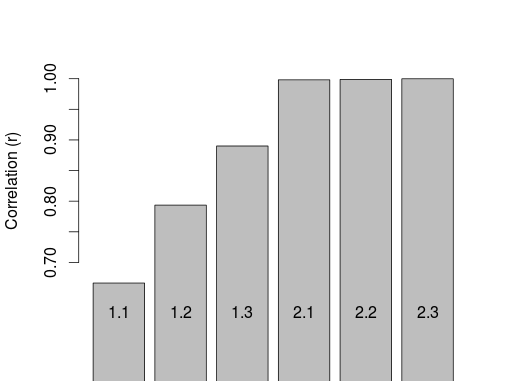
\includegraphics[width=6cm]{corr-baseline}
 \end{center}
\caption{Improvement in goodness of fit with additional constraints and iterations, 
as illustrated by $R^2$ values.}
\label{fnconscor}
\end{figure}

The results for the first 6 constraint-iteration permutations 
of this baseline scenario are illustrated in \cref{fipfinac} and %??? ref
in the online `measures' table. These results show that IPF successfully 
took the simulated cell counts in-line with the census after each constraint 
and that the fit improves with each iteration (only two iterations are 
shown here, as the fit improves very little beyond two).

\begin{figure}
 \begin{center}
  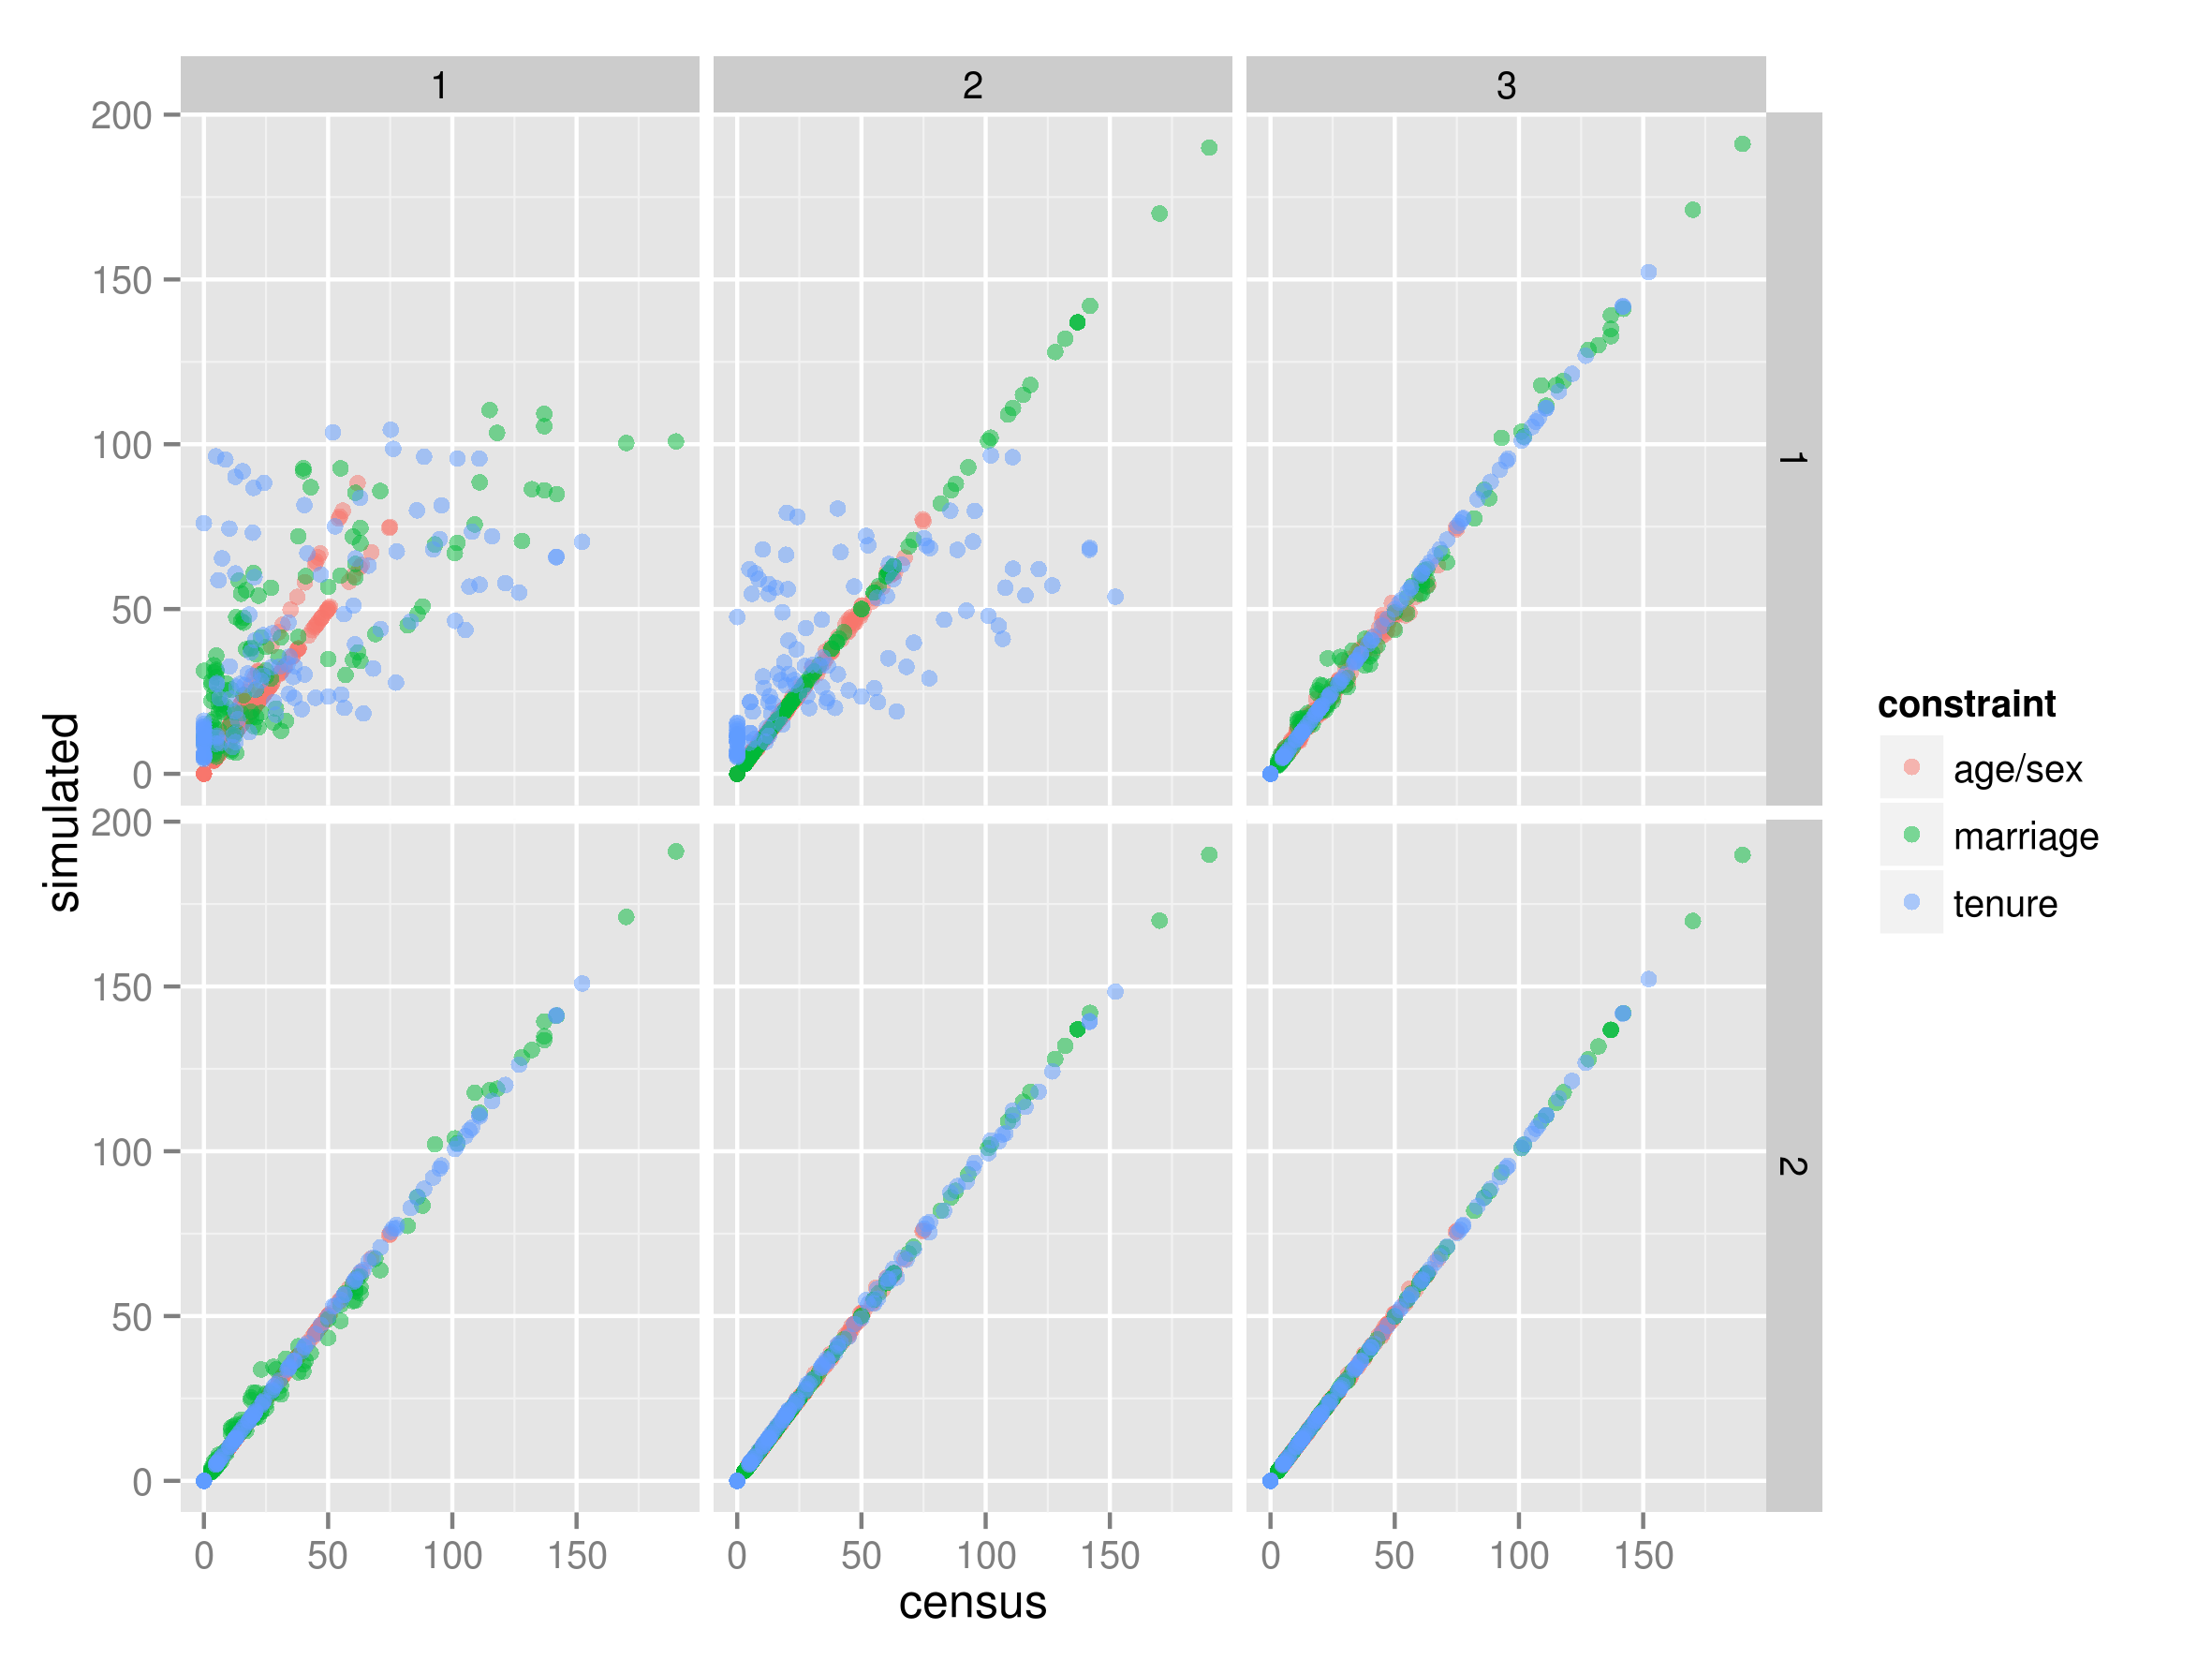
\includegraphics[width=12cm]{ipfinac}
 \end{center}
\caption{IPF in action: simulated vs census zone counts for the small-area baseline scenario after each constraint (columns) and iteration (rows).}
\label{fipfinac}
\end{figure}

Rapid reductions in the accuracy improvement from
additional computation were observed in each scenario, as illustrated
by the rapid alignment of zone/constraints to the 1:1 line in \cref{fipfinac}.
After four iterations, in the `simple' scenarios,
the fit is near perfect, with an $R^2$ value indistinguishable from one
to 7 decimal places. The decay in the rate of improvement with additional 
iterations is super-exponential. 

\subsection{Initial weights}
It was found that initial weights had little impact on the overall simulation. 
Taking the simplest case, a random individual (id = 228) was selected from the 
`small area' data and his/her initial weight was set to 2 
(instead of the default of 1). The impact of this change on the individual's 
simulated weight decayed rapidly, tending to zero after only 5 iterations in the small-area scenario. 
It was found that altered initial weights affect the simulated weights of all other individuals; 
this is illustrated in \cref{ficweight}, which shows the impact on individual 228 and a randomly selected 
individual whose initial weight was not altered, for all areas.

\begin{figure}
 \begin{center}
  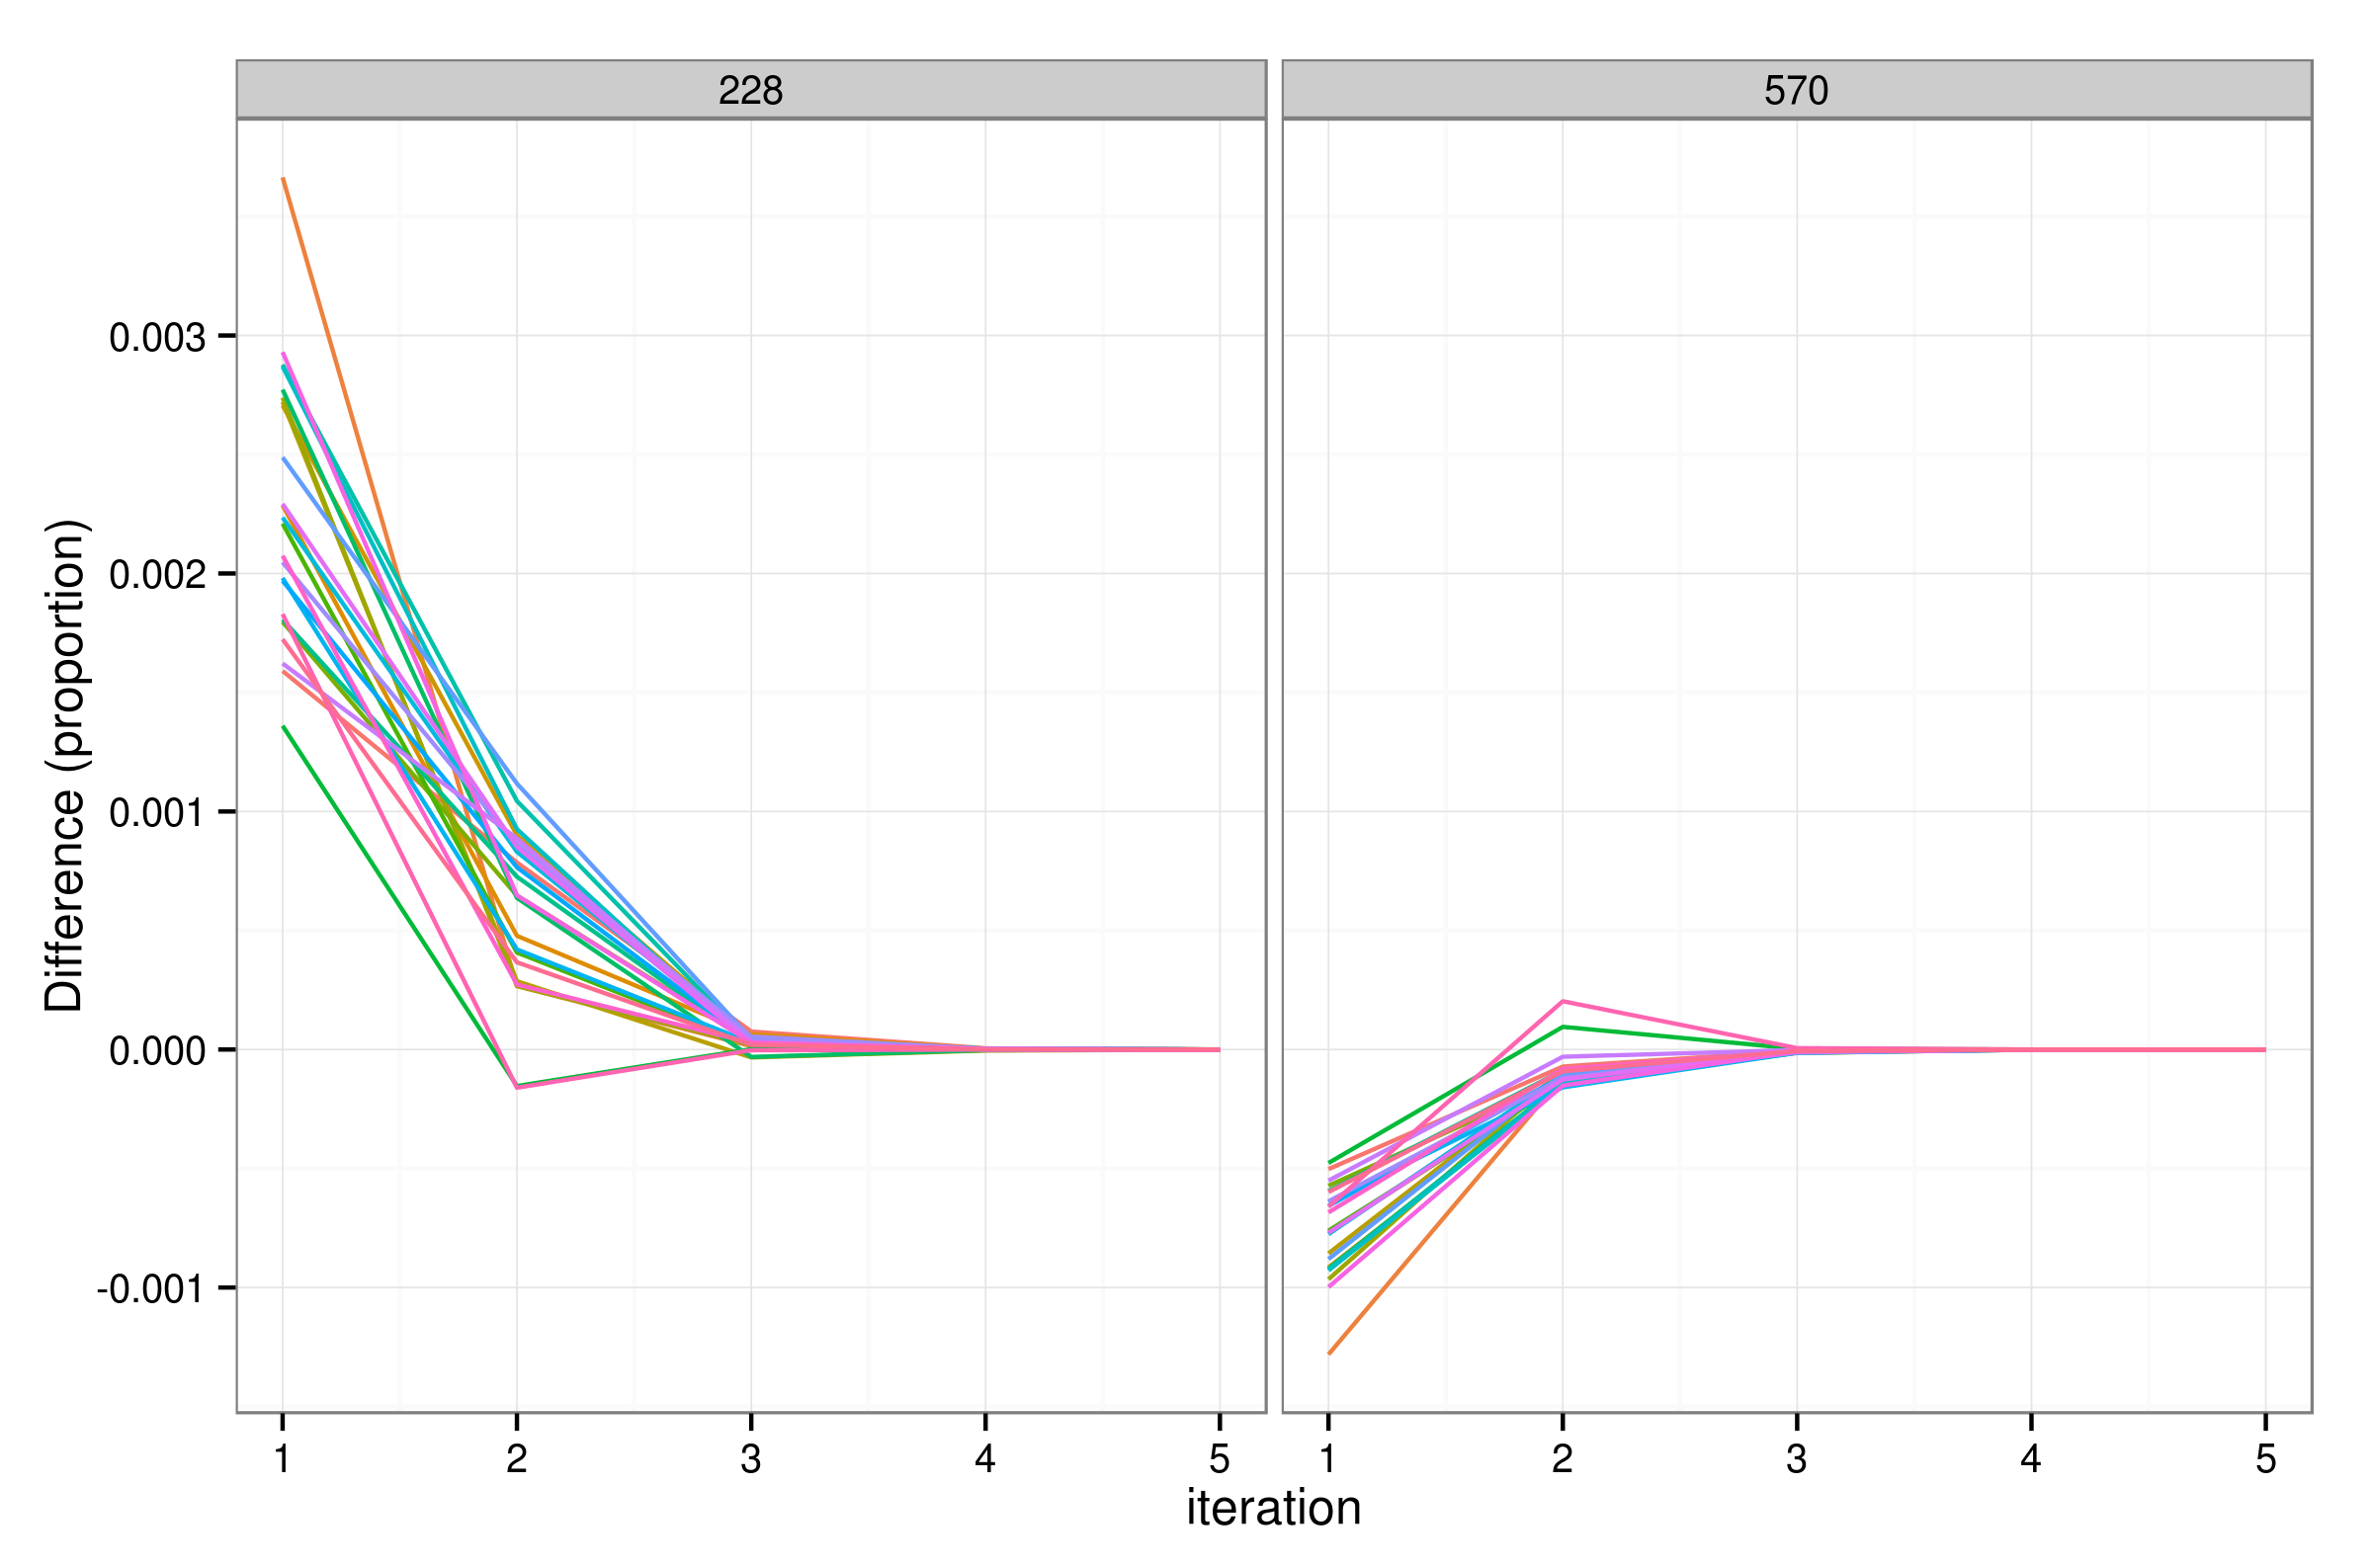
\includegraphics[width=12cm]{weight-1-5-its}
 \end{center}
\caption{The impact of changing the initial weight of individual 228 on the simulated weights of two individuals after 5 iterations. Each of the 24 coloured lines represents a single zone.}
\label{ficweight}
\end{figure}

\cref{ficweight} shows that changing initial weights 
for individuals has a limited impact on the results that
 tends to zero from one iteration to the next. 
After iteration one the impact of a 100\% increase in the initial weight 
of individual 228 had reduced to 0.3\%; after 3 iterations the impact was negligible. 
The same pattern can be observed in the control individual 570, 
although the impact is smaller and in the reverse direction. 
The same pattern can be observed for other individuals, by altering the `analysis.min'.

To analyse the impacts of changing the initial weights of multiple 
individuals, the same experiment was conducted, but this time the initial weights were
applied to the first five individuals. The results are illustrated in \cref{finweight},
which shows the relationship between initial and final weights for the first two individuals
and another two individuals 
(randomly selected to show the impact of altering weights on other individual weights). 

\begin{figure}
 \begin{center}
  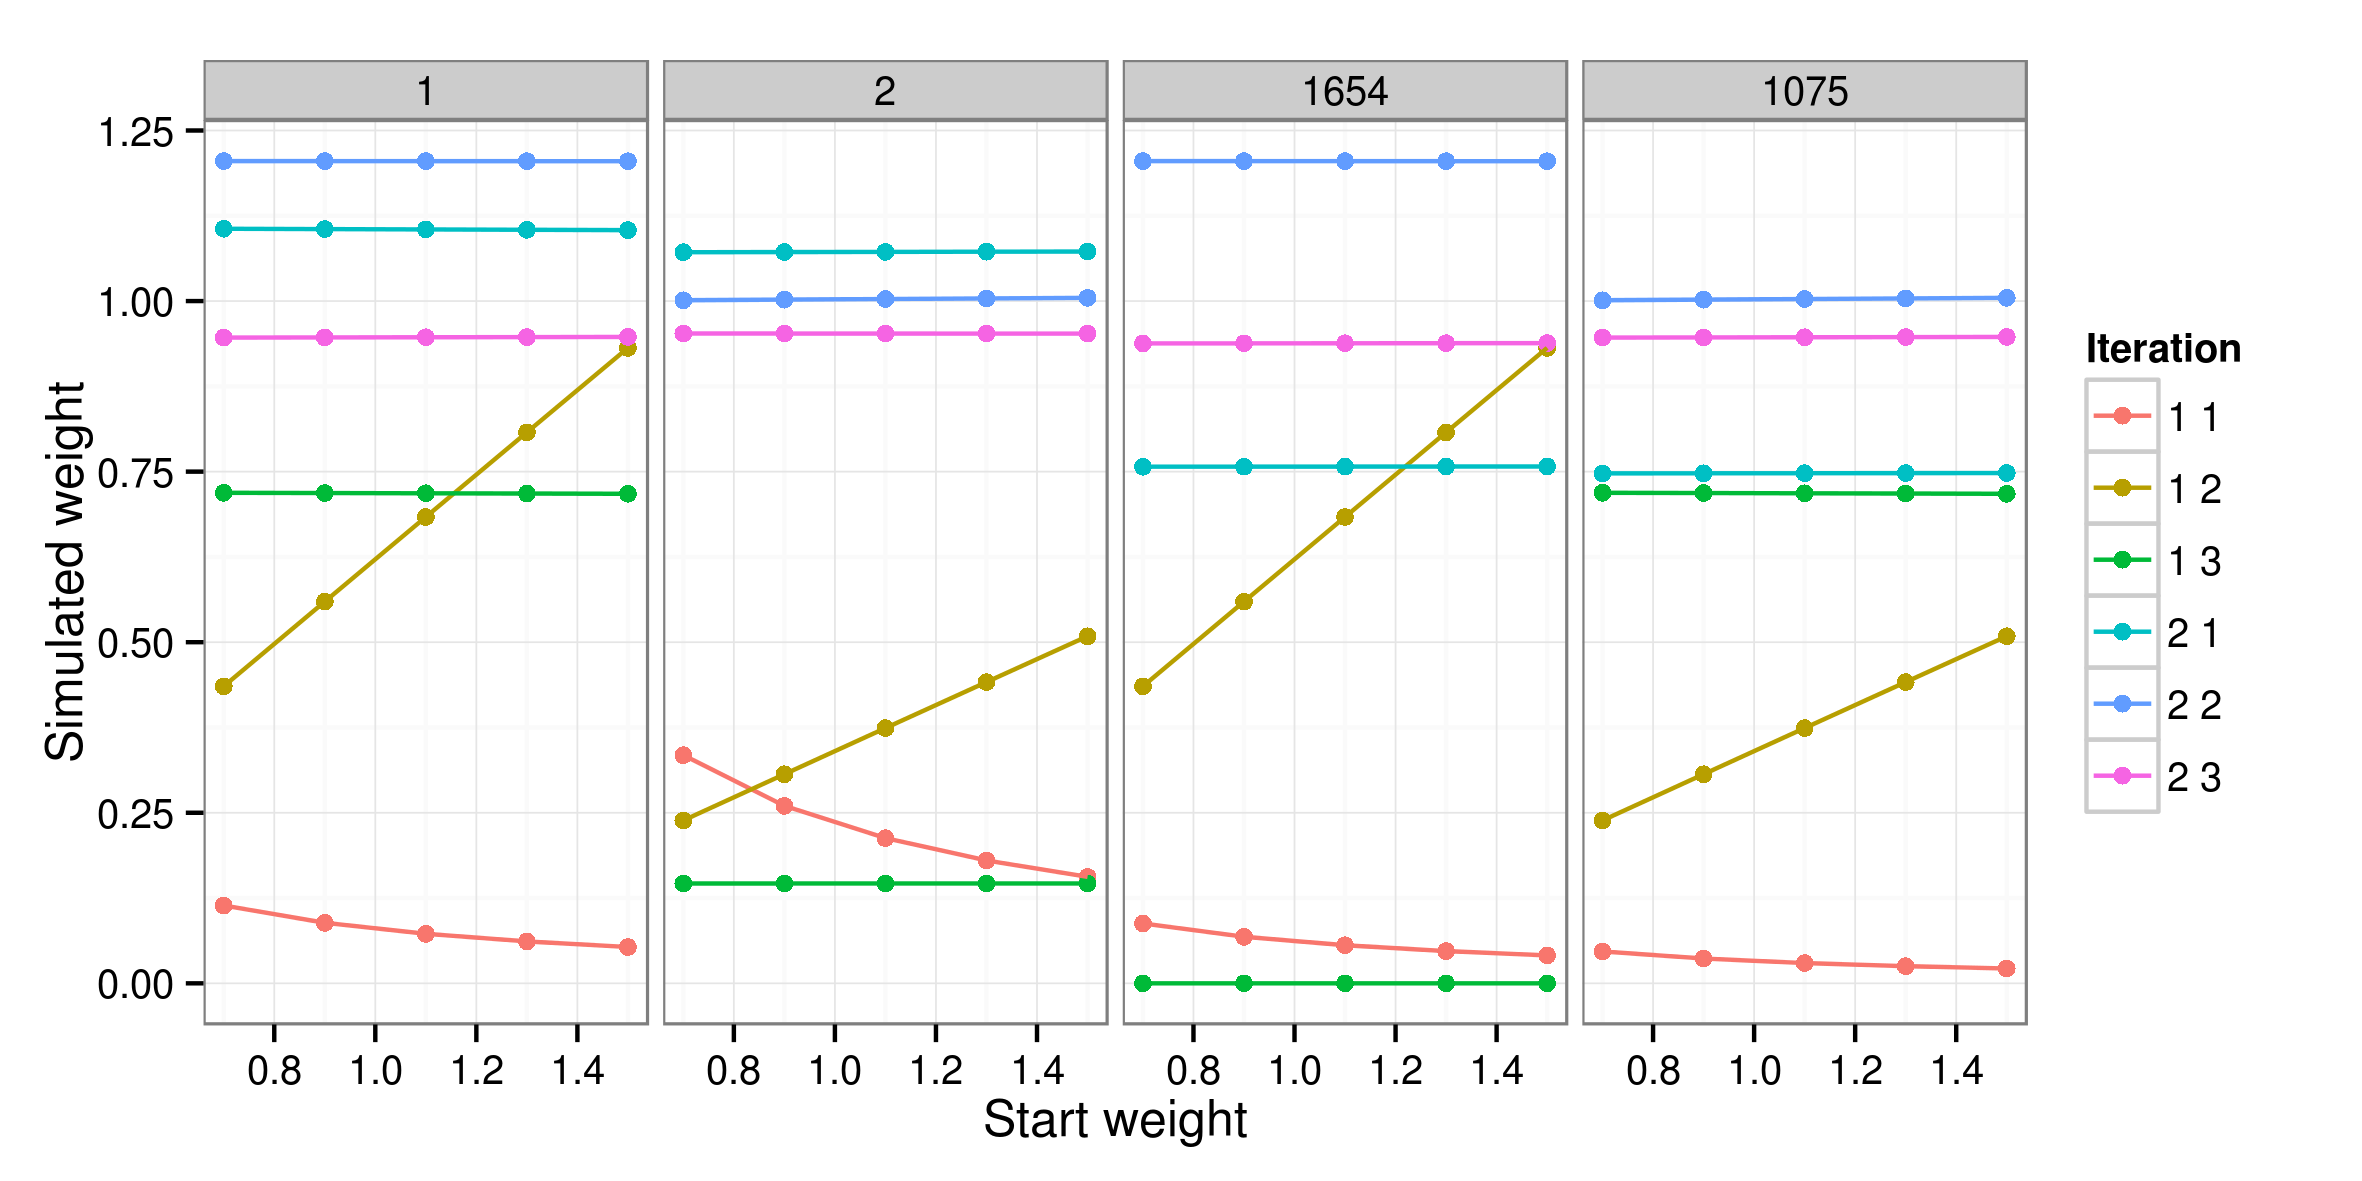
\includegraphics[width=12cm]{weights-exp-54nice2}
 \end{center}
\caption{Initial vs simulated weight of four individuals for a single area (zone 1).}
\label{finweight}
\end{figure}

\cref{finweight} shows that the vast majority of the impact of altered starting weights occurs in iteration-constraint
combinations 1.1 and 1.2, before a complete iteration has even occurred. 
After that, the initial weights continue to have an influence, of a magnitude that cannot be 
seen. For individual 1, the impact of a 53\% difference in initial weights (from 0.7 to 1.5) shrinks to 
2.0\% by iteration 1.3 and to 1.1\% by iteration 2.3. 

These results suggest that initial weights have a limited impact on the results of IPF, that declines rapidly with each iteration. 

\subsection{Empty cells}

There were found to be 62 and 8,105 empty cells in the `small-area' and `Sheffield'
baseline scenarios, respectively. Only the smallest input dataset was
\emph{complete}. Due to the multiplying effect of more variables (\cref{eqempty}),
$Nperm$ was found to be much larger in the complex models, with values rising from
4 to 300 and 9504 for the increasingly complex test examples. 

As expected, it was found that adding additional empty cells
resulted in worse model fit, but only slightly worse fit if few empty
cells (1 additional empty cell to 10\% non-empty cells) were added.
The addition of new rows of data with attributes corresponding
to the empty cells to the input dataset allowed the `small-area' and `Sheffield'
models to be re-run without empty cells. This resulted in substantial improvements in
model fit that became relatively more important with each iteration: model
runs with large numbers of empty cells reached minimum error values quickly, beyond
which there was no improvement.

\subsection{Integerisation}

After passing the final weights through the integerisation algorithms mentioned
in \cref{sintm}, the weight matrices were of identical dimension and total population as
before. It was found that, compared with the baseline scenarios, that integerisation
had a negative impact on model fit.
For the `simple' and `small area' scenarios, the impact of integerisation was proportionally
large, greater than the impact of any other changes. For the more complex Sheffield example,
by contrast, the impact was moderate, increasing RMSE by around 20\%.

\subsection{Computational efficiency} \label{sspeedr}

The times taken to perform IPF in the original R code and the new
low-level C implementation are compared in \cref{tspeed}. This shows that running
the repetitive part of the modelling in a low-level language can have
substantial speed benefits --- more than 10 fold improvements were found for
all but the simplest model runs with the fewest iterations. 
\Cref{tspeed} shows that the computational efficiency benefits of running IPF in C
are not linear: the relative speed improvements increase with the both the
number of iterations and the size of the input datasets.

This suggests two things:
\begin{itemize}
 \item Other parts of the R code used in both the `pure R' and C implementations via \textbf{ipfp}
 could be optimised for speed improvements.
 \item Greater speed improvements could be seen with larger and more complex model runs.
\end{itemize}

% \footnote{`For' loops
%     are notoriously slow in R \citep{Matloff-R}, so their removal from
%     the code could
%     probably further increase the speed of execution.}

\begin{table}[htbp]
\caption{Time taken for different spatial microsimulation models to run in microseconds, comparing
    R and C implementations code. 
    3 (left hand columns) and 10 (right hand columns) iterations were tested for each.
    `Improvement' represents the
    relative speed improvement of the C implementation, via the \textbf{ipfp} package.}
    \begin{center}
\begin{tabular}{lrrrrrr}
\toprule
 & \multicolumn{ 3}{c}{3 iterations} & \multicolumn{ 3}{c}{10 iterations} \\
 Scenario & \multicolumn{1}{l}{R code} & \multicolumn{1}{l}{C code (ipfp)} & \multicolumn{1}{l}{Improvement} & \multicolumn{1}{l}{R code} & \multicolumn{1}{l}{C code (ipfp)} & \multicolumn{1}{l}{Improvement} \\
\midrule
Simple & 73 & 8 & 9.1 & 231 & 8 & 28.9 \\ 
Small-area & 3548 & 204 & 17.4 & 10760 & 288 & 37.4 \\ 
Sheffield & 44051 & 1965 & 22.4 & 135633 & 2650 & 51.2 \\ 
\bottomrule
\end{tabular}
\label{tspeed}
    \end{center}
\end{table}

\subsection{Summary of results}

The impact of each model experiment on each of the three scenarios
is summarised in \cref{tsum}. It is notable that the variable with the
greatest impact on model fit varied from one scenario to the next,
implying that the optimisation of IPF for spatial microsimulation is
context-specific. Changes that had the greatest positive impact on model
fit were additional iterations for the simpler scenarios and the removal of
empty cells from the input microdata for the more complex `Sheffield' scenario.

Likewise, the greatest negative impact on model fit was due to the same variable
for the simpler scenarios: integerisation. For `Sheffield', the
use of only one complete iteration (not shown in \cref{tsum})
instead of 3 or more had the a more damaging impact than any of those presented,
highlighting the importance of performing multiple iterations of IPF.

Substantial improvements in execution speed have been demonstrated using a lower-level
implementation of the IPF algorithm than has been used in previous research.
% New - thanks DL
If computational efficiency continues to increase,
the code could run 100 times faster than current implementations
on larger datasets (see \cref{tspeed}).
% Assuming % old
% computational efficiency benefits continue to increase with more complex datasets,
% as observed in \cref{tspeed} and that further efficiency improvements
% are possible, it is conceivable that
% code more than 100 times faster than a recent
% implementation of IPF \citep{Lovelace2013-trs} could be developed.

\begin{table}[h]
\caption{Summary results of root mean square error (RMSE) between
simulated and constraint data.} \label{tsum}
\begin{center}
\begin{tabular}{llll}
\toprule
Test scenario & Simple & Small area  & Sheffield \\
\midrule
\textbf{Baseline} & 0.0001 & 0.018  & 25.5 \\
\midrule
\textbf{Constraints and iterations} &  &  & \\
1 iteration & 0.221 & 1.91 & 78.2 \\
5 iterations & \textless 0.000001 & 0.00001  & 20.9 \\
10 iterations & \textless 0.000001 & 0.000002  & 13.8 \\
Reordered constraints 		& 0.0001  & 0.018 & 14.5 \\ % it is worse, but only a little!
\midrule
\textbf{Initial weights} 	&  &  & \\
10\% sample set to 10  		& 0.0001 & 0.034  & 25.5\\
10\% sample set to 1000 	& 0.0001 & 0.998 & 25.5 \\
\midrule
\textbf{Empty cells} 		&  &  & \\
1 additional empty cell 	& 0.852 & 0.018  & 25.5 \\
10\% additional empty cells 	& --- & 0.050  & 25.6 \\
No empty cells			& --- & 0.005 & 1.24 \\
\midrule
\textbf{Integerisation} 	&  &  & \\
TRS integerisation		& 0.577 & 3.68  & 29.9 \\
Proportional probabilities & 1.29 & 3.91 & 30.0 \\
\bottomrule
\end{tabular}
\end{center}
\end{table}

\section{Conclusions}
In this paper we have systematically reviewed and tested modifications to the
implementation of the IPF algorithm for spatial microsimulation --- i.e. the creation
of spatial microdata. This is the first time
to our knowledge that such tests have been performed in a consistent and reproducible
manner, that will allow others to cross-check the results and facilitate
further model testing. The model experiments conducted involved changing one of the
following variables at a time:

\begin{itemize}
 \item Order of constraints and number of iterations.
 \item Modification of initial weights.
 \item Addition and removal of `empty cells'.
 \item Integerisation of the fractional weights using a couple of probabilistic methods ---
 `TRS' and `proportional probabilities'.
 \item The language in which the main IPF algorithm is undertaken, from R to C via the \textbf{ipfp} package.
\end{itemize}

% Some of the variables altered !!!
In every case, the direction of change was as expected, confirming
prior expectations about the influence of model set-up on performance. The finding
that the initial weights have very little influence on the results, particularly
after multiple iterations of IPF, is new and relevant to the spatial microsimulation
community. This finding all but precludes the modification of initial weights as
a method for altering IPF's performance and suggests that research time would be
best focused on other variables, notably empty cells.

A new contribution of this paper is its analysis
of empty cells --- individuals absent in the individual-level dataset but
implied by the geographically aggregated constraints.
The methods presented in \cref{smempty} should enable others to
identify empty cells in their input datasets and use this knowledge to
explain model fit or to identify synthetic individuals to add.
This is the first time, to our knowledge, that empty cells have been shown to have
large adverse effect on model fit compared with other variables in model design.

The removal of empty cells greatly improved fit,
especially for complex scenarios. This straightforward change had
the single greatest positive impact on the results, leading to the 
conclusion that removing empty cells can substantially enhance the performance of
spatial microsimulation models, especially those with many constraint variables and relatively
small input input datasets.
On the other hand, a potential downside of removing empty cells is that it involves adding fictitious
new individuals to the input microdata. This could potentially cause problems if the
purpose of spatial microsimulation is small area estimation, where the
value of target variables (e.g.~income) must be set.
Another potential problem caused by removal of empty cells that must be avoided is
the creation of impossible combinations of variables such as car drivers under
the age of 16.

% Despite these concerns, our finding that empty cells has a large impact on model % waffle!
% results is robust across all scenarios and should be taken seriously in future research.
% A direct recommendation from these findings is therefore that researchers should
% test for missing cells, as defined in \cref{smempty}, before reweighting.

The most useful practical finding for future researchers dealing with large spatial microsimulation
models and limited computational resources is likely to relate to computational efficiency.
The implementation
of the IPF procedure in a low-level language via the recently published \textbf{ipfp} package
yielded execution times dozens of times faster than the original R implementation.
The speed benefit of this low-level implementation rose with additional iterations
and model complexity, suggesting that the method of implementation may be more influential than
the number of iterations. Regarding the optimal number of iterations,
there is no magic number identified in this research. However, it is clear that
the marginal benefits of additional iterations decline rapidly: we conclude that 10 iterations
should be sufficient for complete convergence in most cases.
% In any case, the number of iterations becomes much less important
% for the timing of IPF if a low-level implementation is used.
% This finding highlights the importance of software selection
% and code design when working on large datasets.

There are many opportunities for further research raised by this paper.
There is clearly a need for further testing in the area of spatial microsimulation overall,
and we have demonstrated this for the established IPF method. Research questions
raised relating to IPF specifically include:
What are the impacts of constraining by additional variables affecting the performance of IPF?
What are the interactions between different variables --- e.g. what is the
combined impact of altering the number of empty cells \emph{and} number of
iterations simultaneously? Can change in one variable reduce the need for
change in another? What are the opportunities for further improvements in computational efficiency
of the code?

Moreover, there are broader questions raised by this research concerning the validation
of models that are used for policy making. \citet{Scarborough2009} highlight the
paucity of evaluation studies of model-based local estimates of heart disease,
even when these estimates were being widely used by the medical profession for
decision making. We contend that such issues, with real-world consequences, are exacerbated
by a lack of reproducibility, model evaluation and testing
across spatial microsimulation research. The paper's methods --- supplied in
the \href{http://tinyurl.com/lgw6zev}{Supplementary Information} ---
and reproducible results
address these issues, providing new insight into the likely impacts of different
variables on the performance of the IPF procedure. There is however much further
work to be done, including research into external validation, handling of very
large datasets, and grouping output microdata into household units.

% The findings encourage such work and 
% provide a basis for such tests and a baseline for new test procedures.
% 
% The existing literature called
% for increased model testing and validation in spatial
% microsimulation.
% 
% It is in this wider context that our study has clarified
% understandings of the impact of a number of variables on the internal fit of
% one particular method for producing such small area estimates. There is however further work to be done in the area.
% The wider contribution is an illustration of the utility of model testing:
% similar tests applied to other widely used procedures may also yield surprising results,
% with potential benefits for method design across the social sciences.
% In the field of spatial microsimulation, further testing and methodological advance
% will help ensure that the
% models are  researchers who use them and society at large.

\bibliographystyle{model2-names.bst}
\bibliography{/home/robin/Documents/Microsimulation.bib}

%/nfs/foe-fs-01_users/georl/repos/IPF-performance-testing/paper/ipflib.bib  desktop.bib,
% /home/robin/Documents/Microsimulation.bib,
% /home/robin/Documents/powerstarrefs/Microsimulation.bib
% /nfs/foe-fs-01_users/georl/Documents/Microsimulation.bib,

% \section{Appendix: Formulae for evaluation techniques and additional results}
% 
% The symbols used for values in these equations follows, to the
% extent possible, the most common usage found in the literature.
% Thus $T_{ij}$ and $U_{ij}$ represent the simulated and observed
% cell counts for category $i$ in zone $j$. Additional symbols are
% described as and when they appear in the formulae.
% 
% 
% \subsection{Modified Z-Scores}
% 
% The modified Z-score ($Zm$) was described by \citet{Williamson1998}
% and is defined as follows:
%  
% \begin{equation}
%  Zm_{ij} = (r_{ij} - p_{ij}) \Bigg/ \left(\frac{p_{ij}(1 -
% p_{ij}))}{\sum\limits_{ij}U_{ij}}\right)^{1/2}
% \end{equation}
% 
% where
% 
% \begin{center}
% \begin{math}
%   p_{ij} = \frac{U_{ij}}{\sum\limits_{ij}U_{ij}} \qquad and \qquad r_{ij} =
% \frac{T_{ij}}{\sum\limits_{ij}U_{ij}}
% \end{math}
% \end{center}


\end{document}
